\section{Round30: three adaptive investigations}

\label{sec:round30-overview}

Human author: \textbf{Hruday N M (BUNZEEY)}. This cycle contains exactly three reviewed investigations. AT1 was selected from the inherited roadmap; the later contracts were selected only after the preceding evidence and skeptical feedback. Source research, replay, editorial integration and publication do not count as extra investigations.

The current conclusions concern the original Wilson observable in the numerical-cap AQ state. HNM names identify this specific contribution record. Earlier eponyms, authors, physical symbols and frozen evidence remain intact. The three contributions and their separate equation aliases are not three proofs of continuum Yang--Mills.

\section{Round30 source comparison and reading limits}
\label{sec:r30-sources}
The following records describe selected source reading, not an exhaustive state-of-the-art survey. Historical documents, patents, government custody and subreddit discussions may motivate controls, but none establishes a new Hamiltonian term. An unread lead remains a lead. Standard methods and their authors retain attribution.
The modern comparison uses moment duality of Bertsimas--Popescu~\citep{bertsimas2005moments} and the spectral-kernel formulation of Abbott and collaborators~\citep{abbott2026causal}. These precede this application. The positive pointwise certificates in the following derivations do not claim a new generic moment method. The magnetic-basis trial-state route of Spriggs and collaborators~\citep{spriggs2025su2} remains prospective; finite numerical energy improvements do not prove a lower gap.
\begingroup\footnotesize\setlength{\tabcolsep}{4pt}
\begin{longtable}{@{}p{43mm}p{65mm}p{44mm}@{}}
\toprule Source / version & Actual reading and relevance & Limits\\\midrule\endhead
\href{https://arxiv.org/html/2503.15539v3}{Pinched Multi Affine Geometry and Confinement: Describing the Yang--Mills Mass Gap}\par v3, 2026-09-14; v1 2025-03-06; v2 2026-09-11 & Selected statements and adjacent explanation; not entire paper\par Abstract and version history; II.3 Proposition 2.4; II.4 Theorem 2.5 and Corollary 2.6; Proposition 2.7\par Closest prior comparison for AQ construction and a proposed spectral-response follow-up. & No wholesale validation of all manuscript claims; no scientific-priority determination.\\\addlinespace
\href{https://arxiv.org/src/2503.15539v3/anc/PinchedMultiAffineGeometry_Supplement.pdf}{Pinched Multi Affine Geometry: supplementary proofs}\par v3 ancillary supplement, 2026-09-14 & Targeted proof passages, printed S6-S8; no whole-supplement audit\par A.9 excitation-energy passage; A.10 local compactness, dynamics, GNS continuity and spectral passage; A.11 proof of Corollary 2.6\par Prevents renaming the generic strategy as an HNM invention. & AQ group, reference factors, seven-star region and constants require their own proofs.\\\addlinespace
\href{https://www.claymath.org/wp-content/uploads/2022/06/yangmills.pdf}{Quantum Yang--Mills Theory: the Clay problem statement}\par Official Clay-hosted problem statement; URL directory 2022/06 is not treated as publication date & Targeted pages 5-6 of PDF\par Section 3 Quantum Fields; Section 4 The Problem; Beginning of Section 5 Comments\par Scope gate for all fixed-spacing workbench claims. & The workbench has not constructed the required continuum fields.\\\addlinespace
\href{https://arxiv.org/pdf/1410.8174}{On the dynamics of lattice systems with unbounded on-site terms in the Hamiltonian}\par v1, 2014-10-29 & Targeted theorem and assumptions\par Section 3 countable metric lattice and summability/convolution hypotheses; Theorem 4.1 and beginning of its proof\par Actual AQ dynamics ancestry; limit in volume and continuity in time are distinct. & No new reproof of the external theorem; actual matching is inherited from AQ1.\\\addlinespace
\href{https://arxiv.org/abs/1810.02428v2}{Quasi-Locality Bounds for Quantum Lattice Systems, Part I}\par v2, 2019-03-01; J. Math. Phys. 60, 061101 (2019) & Metadata and abstract only in this pass\par Abstract and version history\par Further theorem route; not a replacement for the explicitly checked NS theorem. & Specific NSY theorem transfer not checked anew.\\\addlinespace
\href{https://math.ucr.edu/home/baez/penrose/Penrose-AngularMomentum.pdf}{Angular momentum: an approach to combinatorial space-time}\par 1971, Quantum Theory and Beyond, original pp.151-180; hosted transcription & Selected opening passages; later combinatorial rules not audited\par PDF pages 1-6: opening motivation, spin labels, model caveat, relational-angle proposal\par Inspires representation and inner-product checks, not a mass-gap premise. & No transfer of emergent geometry into the workbench model; no endorsement.\\\addlinespace
\href{https://calteches.library.caltech.edu/51/2/CargoCult.htm}{Cargo Cult Science}\par 1974 Caltech commencement address & Full short web text inspected; this ledger paraphrases only the named passages\par Opening mystical-experience discussion; Integrity and disconfirming details paragraphs; Publishing unfavorable outcomes; Baseline replication discussion\par Discriminating controls and source-qualified novelty; personal experiences do not establish physical mechanisms. & Historical anecdotes were not independently investigated; no physical conclusion relies on them.\\\addlinespace
\href{https://feeds.library.caltech.edu/people/Feynman-R-P/article.html}{Simulating physics with computers: bibliographic lead}\par 1982 article metadata, Int. J. Theor. Phys. 21, 467-488 & Metadata only; linked resolver produced retrieval error\par Simulating physics with computers bibliographic entry\par Lead retained without pretending full-text reading. & Article text unread in this pass.\\\addlinespace
\href{https://arxiv.org/html/2509.12323v1}{Accurate ground states of SU(2) lattice gauge theory in 2+1D and 3+1D}\par v1, 2025-09-15 & Selected model/ansatz sections and code-availability statement\par Abstract; II.1 Hamiltonian and representation; II.2 Variational model; V Code and data availability\par Concrete future AS reference strategy preserving the actual coupling dictionary. & Code not installed or run; variational values do not certify a lower spectral gap.\\\addlinespace
\href{https://arxiv.org/html/2607.26132v1}{Untruncated SU(2) theory with dynamical fermions: selected author preprint}\par v1, 2026-07-28 & Selected technical model passages, not numerical validation\par Abstract; Model paragraph and Eqs.(1)-(2); Variational wavefunction description\par Model-deformation warning and current simulation lead. & Different dimension and matter content from AQ; numerical conclusions not independently reproduced.\\\addlinespace
\href{https://arxiv.org/html/2507.16890v2}{Finite-temperature spectral functions in the lattice Schwinger model: selected author paper}\par v2, 2025-12-09; Phys. Rev. D 112, 114505 (2025) & Selected response definitions and numerical-scope passages\par Lattice Schwinger model setup; Spectral functions subsection Eqs.(10)-(13); Finite-lattice peak/width qualification paragraphs\par Operational spectral-response design and resolution warning. & Not the AQ model; no spectral pole or continuum inference transfers automatically.\\\addlinespace
\href{https://web.mit.edu/dbertsim/www/papers/MomentProblems/Optimal-inequalities-in-probability-theory-A-convex-optimization-approach-SIAM15.pdf}{Optimal Inequalities in Probability Theory: A Convex Optimization Approach}\par SIAM J. Optim. 15(3),780-804 (2005), DOI 10.1137/S1052623401399903; paper states electronic publication 2005-04-08 & Selected formulation and proof passages; no whole-paper reproduction\par Section 2, dual problem, upper-moment sign rule, Theorems 2.1-2.2; Section 3, Proposition 3.1 positivity certificates\par Closest classical method for prospective Loop2; no generic novelty claim. & No claim of strong duality or optimality for workbench certificates.\\\addlinespace
\href{https://arxiv.org/html/2605.20509v1}{The Causal Bootstrap: Bounding Smeared Spectral Functions from Non-Perturbative Euclidean Data}\par v1, 2026-05-19 & Selected method and interpretation passages; no numerical reproduction\par III.1 dual exact-data certificates; IV.1-IV.3 rational and piecewise polynomial kernels; VII.4 distinction between extremal spectra and true spectrum; VIII kernel and positivity caveats\par Direct current prior overlap for proposed response bounds; exact arithmetic recommended for this small case. & No imported stochastic covariance or all-results validation; AQ inputs are deterministic analytic bounds.\\\addlinespace
\href{https://newton.dlib.indiana.edu/text/ALCH00017/normalized}{Keynes MS.28: Hermes / Tabula Smaragdina}\par Indiana University normalized transcription & Metadata and English ff.2r--2v read; Latin commentary visible but not fully translated; manuscript images not collated\par ff.2r--2v: above/below correspondence and separation/recombination; catalogue distinction between English translation, Latin transcription and commentary\par Ask for an explicit state/generator/scale map before identifying theories. & No complete Latin commentary translation or manuscript collation\\\addlinespace
\href{https://newton.dlib.indiana.edu/text/ALCH00109/normalized}{Add.3973: Experiments}\par Indiana University normalized transcription & Metadata; ff.1r--2r and ff.5r--6r read; no complete notebook claim\par December 1678 residues and mixtures; January 1679/80 uncertain dry weights, cracked vessel and escaped material\par Keep actual residual, omitted-channel and state-replacement costs in AT/AU certificates. & Modern chemical identities and reproducibility not investigated\\\addlinespace
\href{https://patents.google.com/patent/US787412A/en}{US787412A: Art of transmitting electrical energy through the natural mediums}\par Patent text mirrored by Google Patents & Description of terrestrial standing waves, three resonance requirements and receiving apparatus read; no physical performance validation\par Diameter/quarter-wave condition and approximate six-per-second lowest rate; Duration requirement; Tuned receiver and location-dependent zero response at nodes\par Specify the full generator, source, receiver and null geometry; do not equate a measured peak with a unique eigenvalue. & OCR not collated against original patent image; no performance audit\\\addlinespace
\href{https://www.ramakrishnavivekananda.info/vivekananda/volume_5/epistles_first_series/057_blessed_and_beloved.htm}{Letter to E. T. Sturdy, 13 February 1896}\par Complete Works V, Epistles First Series LVII in this transcription & Letter text read, with attention to Tesla paragraph and cosmology discussion\par Tesla's reported interest in Prana, Akasha and Kalpas; Expected later mathematical demonstration; Vivekananda's cosmological interpretation\par Separate promised unification from a supplied mathematical map. & No original manuscript facsimile collated; demonstration not located\\\addlinespace
\href{https://www.gutenberg.org/files/48225/48225-h/48225-h}{Collected Papers on Analytical Psychology}\par Authorized translation, second edition reprinted; Project Gutenberg ebook 48225 & Title/edition, author's second-edition preface and Chapter I Automatisms pp.50--54 read; later synchronicity works not read here\par 1917 preface distinction between subject's numerical associations and author's explanation; Automatisms: experimenter cueing, table responses, and meaningless outputs preceding interpreted ones\par Freeze tests and selection rules; retain null outputs and distinguish observed data from interpretation. & No modern clinical evaluation; no claim to survey all Jung writings\\\addlinespace
\href{https://scientific-info.cern/archives/Pauli_archive/guide/letters}{The Pauli Letter Collection}\par CERN collection guide CERN-ARCH-PLC & Collection scope, archival history, finding aids and allied materials read\par CERN collection includes philosophical, psychological and epistemological correspondence; Pauli--Jung correspondence is held in ETH's Pauliana collection\par Trace claims to the correct document and correspondent before interpreting them. & Letter 1417 from Pauli to Fierz, 1952-06-03, is an unread lead; its CDS page returned an anti-bot interstitial\\\addlinespace
\href{https://www.reddit.com/r/occult/comments/1iv5hyv/nikola_tesla_with_his_equipment_for_producing/}{Nikola Tesla, with his equipment for producing high-frequency alternating currents}\par Public Reddit thread as retrieved 2026-09-22 & Opening post and first displayed replies; no representative forum sample\par Post's Tesla/Solfeggio/528 Hz/consciousness connection; Author's link to an original musical composition\par Reject the jump from an emotionally salient or resonant output to its alleged physical cause without a model and control. & Attributed quotation not authenticated; physical or physiological claim not tested\\\addlinespace
\href{https://vault.fbi.gov/nikola-tesla/Nikola%20Tesla%20Part%2003%20%28Final%29/view}{Nikola Tesla Part 03 (Final)}\par Official FBI release catalogue and linked 64-page PDF & Catalogue and PDF metadata only; text extraction empty; requested page screenshots produced text-only placeholders and were not visually inspected\par Catalogue title and download description\par Distinguish documentary custody from experimental confirmation. & Underlying pages remain unread; no claim regarding death rays, energy technology or hidden equations\\\addlinespace
\href{https://dlmf.nist.gov/3.5}{NIST DLMF: Quadrature, trapezoidal rules}\par Online reference as read 2026-09-22; no release-version claim & Selected rule definitions and error formulas; no whole-chapter review\par Section 3.5(i); Equations 3.5.1--3.5.3 and adjacent definitions\par Standard trapezoidal rule and convex-error sign; the integrated derivative estimate is derived explicitly in the workbench application. & No novel general quadrature method or optimality claim. Actual AQ Euclidean samples have not been computed.\\\addlinespace
\bottomrule\end{longtable}\endgroup
\repo{research/round30/experts/modern/sources.json}
\par\repo{research/round30/experts/historical/sources.json}


\clearpage\section{Hruday AT1: reviewed admission}

\label{stmt:AT1}

\textbf{Verdict: accepted within scope.} In the actual numerical-cap AQ state at either sign of $|\tau|\le10^{-8}$, the centered original Wilson vector satisfies $\chi\in D(H_{\rm phys})$. Its second-energy moment is at most $\alpha^2(36+98|\tau|)<37\alpha^2$, and its first-energy moment equals $\alpha\omega_{\rm num}(1-W^2)$.

\subsection*{Limits and independent review}

The producer reports were frozen separately before exchange. Their common ancestry, contract and inherited methods remain disclosed. The skeptic reviewed both proofs and executed controls; this does not constitute external human peer review.

\begin{itemize}

\item No equality of finite-to-infinite second moments

\item No AQ/AO/AN state identification

\item No particle pole, exact mass or dispersion

\item No uniqueness of all thermodynamic states or whole-sequence convergence

\item No continuum Yang-Mills construction

\item Scientific priority unverified; established methods retain attribution

\end{itemize}

\repo{research/round30/advisor/at1-gate.json}

\par\repo{research/round30/skeptic/at1.md}

\subsection*{Substantive directional differences}

\begin{itemize}

\item Both directions recover the same coefficient. The reverse checker separately tests inverse-link derivative signs through U \(U^{-1}\); agreement uses shared inherited premises and proof patterns.

\end{itemize}

\clearpage\hypertarget{r30-at1-forward-hruday-same-state-wilson-energy-certificate-at1-forward}{%
\section{Hruday AT1: same-state Wilson energy certificate (forward derivation)}\label{r30:at1:forward:r30-at1-forward-hruday-same-state-wilson-energy-certificate-at1-forward}}

\begin{quote}\small\textbf{Source-bound forward derivation.} This is the complete typeset mathematical report of one producer. Prospective claims describe its original freeze; the shared reviewed result and permitted refinements are stated in the admission section. The two agents share inherited premises and model ancestry. This is neither an independent physical observation nor external human peer review.\end{quote}
Human project author: \textbf{Hruday N M (BUNZEEY)}. AI-assisted independent forward derivation, before reading any current AT1 reverse or skeptic solution. HNM labels below are traceable project aliases; established identities and external authors retain their names. Scientific priority is unverified. This is a model-specific extension, with no new axiom.

\textbf{Result.} In the actual AQ1 chosen subsequential centered-full-Z3 state at either sign of \(|\tau|\le 10^{-8}\), let \(H=H_{\mathrm{num}},phys\), \(\chi=(\pi(W)-\omega_{\mathrm{num}}(W))\Omega\), where W is the original xz plaquette. Then

\begin{equation}
\hnmfit{\chi\in D(H),\qquad
\|H\chi\|^2\le B_2:=\alpha^2(36+98|\tau|)<37\alpha^2,
\qquad
\langle\chi,H\chi\rangle=\alpha\omega_{\rm num}(1-W^2).}
\tag{HNM-AT1-F01}\label{r30:at1:forward:eq1}
\end{equation}

This closes these obligations in AQ's own state without identifying it with AO's orthant state. Second-moment equality is not proved. The actual AQ gap and variance remain inherited hypotheses, not recomputed discoveries.

\hypertarget{r30-at1-forward-model-source-scales-and-proof-dependencies}{%
\subsection{Model, source, scales and proof dependencies}\label{r30:at1:forward:r30-at1-forward-model-source-scales-and-proof-dependencies}}

Use exactly the AQ1 subsequence of whole-star centered boxes \(\Lambda_N=[-N,N]^{3}\) and the same fixed repeated selected coefficient triple. Every factor owns all 24 positive links whose tail is \((4b_x+r,2b_y+s,b_z)\), \(0\le r<4,0\le s<2\). Both tail and head gauge actions remain. Write

\begin{equation}
\hnmfit{H_N^{raw}=\alpha\sum_{e\;owned}C_e+V_{sel,N}
-\frac{\alpha\tau}{24}\sum_{b+S\subset\Lambda_N}\sum_{f\in O_b}W_f,
\quad S=\{0,e_x,e_y,e_z\},\quad |O_b|=21.}
\tag{HNM-AT1-F02}\label{r30:at1:forward:eq2}
\end{equation}

\(C_e=-\sum_aX_{ea}^2\), with generators \(i \sigma_a/2\). The selected potential is \(-\sum \lambda_f W_f\), with per-factor absolute coefficient budget at most \(9\alpha/8\). With the actual selected-reference ground scalar \(B_N=\sum_b E_{\mathrm{strip},b}\) and \(\delta=\alpha/8\),

\begin{equation}
\hnmfit{\delta\widehat H_N=H_N^{raw}-B_N,\quad
E_N^{raw}=B_N+\delta\widehat E_N,\quad
K_N=H_N^{raw}-E_N^{raw}=\delta(\widehat H_N-\widehat E_N).}
\tag{HNM-AT1-F03}\label{r30:at1:forward:eq3}
\end{equation}

The normalized interaction per anchor obeys \(\|\phi_b\|\le 7|\tau|\). All these terms, including selected bridges and both ground scalars, are retained. Alpha, hbar, lattice spacing and the positive comparison E\_star are fixed. Tau is an interaction coefficient. L below is a proof energy cutoff, not a modified Hamiltonian; no new free physical variable is introduced.

AQ1 supplies local trace-norm convergence along its chosen subsequence, norm convergence of bounded-local dynamics uniformly on compact physical-time intervals, and the actual strongly continuous GNS time group. AQ2 identifies the full physical reducing sector and gives \(H\ge \alpha/16\) on its vacuum orthogonal complement. No AO state limit or old symbolic smallness interval is imported. AO1/AO2 are disclosed shared proof patterns only.

The closest inspected primary comparison is Gauvin~\citep{gauvin2026}, arXiv:2503.15539v3 Supplement A.9-A.11 (saved pp.S6-S8): compactness, centered Fourier transfer, local Wilson first-energy control and spectral-envelope methods already occur there for another model. Nachtergaele-Sims arXiv:1410.8174 is the dynamics theorem already matched in AQ1. Here the specific contribution is the complete SU(2) seven-star commutator estimate and its first-moment/domain conclusion in the actual AQ state. This does not claim invention of spectral uniform integrability or establish priority. Live abstract/version pages were rechecked; reading depth is recorded in inputs/reading.json.

Newton analysis/synthesis guides reconstructing the necessary local energy bound and deriving the limiting statement; Tesla energy accounting guides retaining every gradient channel and scalar. These are modern methodological uses, not claims that those historical people supplied or reviewed this proof. Historical/esoteric interpretations add no premise.

\hypertarget{r30-at1-forward-exact-region-and-seven-star-reset}{%
\subsection{Exact region and seven-star reset}\label{r30:at1:forward:r30-at1-forward-exact-region-and-seven-star-reset}}

The original observable is

\begin{equation}
\hnmfit{W=\tfrac12\operatorname{Tr}[U_{0,x}U_{e_x,z}U_{e_z,x}^{-1}U_{0,z}^{-1}].}
\tag{HNM-AT1-F04}\label{r30:at1:forward:eq4}
\end{equation}

Its four stored links have owners \(0,0,e_z,0\). Its complete-factor cover is \(R=\{0,e_z\}\), containing 48 distinct links. A single factor has eight tails and outgoing slabs of sizes 2,4,8, hence 22 distinct endpoints. For the two stacked factors the tail block has 16 vertices and outgoing slabs of sizes 4,8,8, hence 36 endpoints. These are the original shared endpoint actions; blockwise physical tensor factors are not substituted.

Every incident anchor lies in the exact set

\begin{equation}
\hnmfit{R-S=\{0,-e_x,-e_y,-e_z,e_z,e_z-e_x,e_z-e_y\}.}
\tag{HNM-AT1-F05}\label{r30:at1:forward:eq5}
\end{equation}

All seven whole stars are retained once N\textgreater=2. In the positive orthant only \(0,e_z\) survive, giving the discriminating two-star control. The bulk proof must use seven.

Reset the finite ground density on R to the actual selected-reference rank-one product P\_R, preserving the exterior reduced density. The reset has zero reference energy on R and leaves exterior reference expectations unchanged. Each incident retained interaction changes by at most \(2\|\phi_b\|\le 14|\tau|\). Positivity and the finite full-ground variational principle give

\begin{equation}
\hnmfit{\omega_N(h_R)\le98|\tau|,\qquad h_R=h_0+h_{e_z}.}
\tag{HNM-AT1-F06}\label{r30:at1:forward:eq6}
\end{equation}

The mixed trial need not be gauge invariant because the AQ/AM full ground is the minimum used. All reference terms have finite expectation in the finite ground; replacing only finitely many factors by reference ground vectors keeps finite form energy. Nonnegative spectral truncations justify cancellation of unchanged exterior expectations. This reproduces the regional argument in the actual centered Hamiltonian; it is not a limit-state identification.

Define \(T_R=\alpha\sum_{e\text{ owned by }R}C_e\), \(V_R^{\mathrm{sel}}=-\sum_{f\text{ selected}}\lambda_f W_f\), and \(B_R=\sum_{b in R}E_{\mathrm{strip},b}\). Exactly,

\begin{equation}
\hnmfit{T_R=\delta h_R-V_R^{\mathrm{sel}}+B_R.}
\tag{HNM-AT1-F07}\label{r30:at1:forward:eq7}
\end{equation}

The Haar trial has zero electric and selected Wilson means, so each \(E_{\mathrm{strip},b}\le 0\). The selected absolute budget on R is at most \(9\alpha/4\). Consequently

\begin{equation}
\hnmfit{\omega_N(T_R)\le\alpha\left(\frac94+\frac{49}{4}|\tau|\right).}
\tag{HNM-AT1-F08}\label{r30:at1:forward:eq8}
\end{equation}

Discarding the nonpositive B\_R only after this exact reconstruction is valid. Setting it to zero in the identity is not. The selected-reference ground is generally not Haar: for one nonzero selected plaquette, the trial \(1+tW\) has energy numerator \(3\alpha t^{2}/4-\lambda t/2\), negative at \(t=\lambda/(3\alpha)\). At tau=0 reference energy is zero but actual electric energy need not be zero.

\hypertarget{r30-at1-forward-finite-domains-inverse-links-and-the-full-commutator}{%
\subsection{Finite domains, inverse links and the full commutator}\label{r30:at1:forward:r30-at1-forward-finite-domains-inverse-links-and-the-full-commutator}}

For each finite box, its manifold is the compact product SU(2)\^{}L. The elliptic Casimir sum has Sobolev operator domain H\^{}2 and form domain H\^{}1. The real smooth bounded magnetic multiplication is a bounded perturbation, preserving these domains. Finite ground vectors belong to H\^{}2 (indeed elliptic regularity makes them smooth). Smooth multipliers W,W\^{}2 and their centered versions preserve H\textsuperscript{2/H}1 by the weak product rule and compactness. Thus \(\chi_N=(W-m_N)\Omega_N\) belongs to D(K\_N), with \(m_N=\omega_N(W)\). This is a finite-volume domain result, not an assumed infinite-volume one.

All magnetic multipliers and ground scalars commute with W. For any smooth u,

\begin{equation}
\hnmfit{[C_e,W]u=(C_eW)u-2\sum_a(X_{ea}W)X_{ea}u.}
\tag{HNM-AT1-F09}\label{r30:at1:forward:eq9}
\end{equation}

Each of the four stored link occurrences contributes \(C_eW=3W/4\). To check both orientation and normalization, write its SU(2) holonomy as a quaternion \((w,v)\). Half-Pauli left multiplication gives scalar derivative \(-v_a/2\), so its summed squared derivatives are \((1-w^{2})/4\). For a positive occurrence \texttt{Q=LUR}, the basis is conjugated by L. For an inverse occurrence \(Q=LU^{-1}R\), differentiating \((\exp(tT_a)U)^{-1}\) gives \(-U^{-1} T_a\); on Q this is right multiplication by \(-Ad_{R^{-1}}T_a\). Adjoint rotations preserve the summed squares, and the inverse sign/side remain in the actual derivative. Also \(T_a^{2}=-I/4\) on either occurrence. Hence on all four distinct original links,

\begin{equation}
\hnmfit{\sum_{e,a}(X_{ea}W)^2=1-W^2,\qquad
\sum_e C_eW=3W.}
\tag{HNM-AT1-F10}\label{r30:at1:forward:eq10}
\end{equation}

No other link derivative contributes. Define \(Z_N=\sum_{e in p,a}(X_ea W)X_ea \Omega_N\). Ground centering and (F09) give the L\^{}2 identity

\begin{equation}
\hnmfit{K_N\chi_N=3\alpha W\Omega_N-2\alpha Z_N.}
\tag{HNM-AT1-F11}\label{r30:at1:forward:eq11}
\end{equation}

The derivative cross term is generally nonzero. Pointwise Cauchy-Schwarz and positivity of the four-link electric form inside the complete R sum yield

\begin{equation}
\hnmfit{\|Z_N\|^2\le\int(1-W^2)\sum_{e\in p,a}|X_{ea}\Omega_N|^2
\le\omega_N(T_R)/\alpha.}
\tag{HNM-AT1-F12}\label{r30:at1:forward:eq12}
\end{equation}

Using \(\|W \Omega_N\|\le 1\) and \(\|u+v\|^2\le2\|u\|^2+2\|v\|^2\) now gives

\begin{equation}
\hnmfit{\int E^2d\nu_N(E)=\|K_N\chi_N\|^2
\le18\alpha^2+8\alpha\omega_N(T_R)
\le\alpha^2(36+98|\tau|)=B_2.}
\tag{HNM-AT1-F13}\label{r30:at1:forward:eq13}
\end{equation}

At the exact cap, \(B_2/\alpha^{2}=1800000049/50000000<37\). The estimate is volume uniform along the actual AQ boxes for both tau signs and all allowed selected coefficients. Its units are energy squared; the analogous frequency moment is divided by hbar\^{}2.

\hypertarget{r30-at1-forward-finite-first-energy-identity}{%
\subsection{Finite first-energy identity}\label{r30:at1:forward:r30-at1-forward-finite-first-energy-identity}}

Let \(f_N=W-m_N\). Subtract the weak ground equation tested on \(f_N^{2} \Omega_N\) from the quadratic form evaluated on \(f_N \Omega_N\). The valid H\^{}1 product identities give, for every X,

{\small\path{|X(f_N Omega_N)|^2-Re(conj(X Omega_N) X(f_N^2 Omega_N))=(Xf_N)^2|Omega_N|^2}}.

All potential and scalar terms cancel because they commute with f\_N. Thus, in the actual ground rather than a Haar substitute,

\begin{equation}
\hnmfit{\int E\,d\nu_N(E)=\langle\chi_N,K_N\chi_N\rangle
=\alpha\omega_N(1-W^2).}
\tag{HNM-AT1-F14}\label{r30:at1:forward:eq14}
\end{equation}

Equivalently the double commutator has bounded extension \(2\alpha(1-W^{2})\) and its ground expectation is twice this energy. The factor one half is essential. At the entirely free corner the exact variance is 1/4, Wilson excitation energy 3alpha, first moment 3alpha/4 and second moment 9alpha\^{}2/4. That corner is a normalization fixture only.

\hypertarget{r30-at1-forward-actual-aq-spectral-test-convergence}{%
\subsection{Actual AQ spectral-test convergence}\label{r30:at1:forward:r30-at1-forward-actual-aq-spectral-test-convergence}}

AQ provides local trace-norm state convergence and actual dynamics \texttt{T\_t=lim\_N\ exp(it\ K\_N/hbar)(.)exp(-it\ K\_N/hbar)} in norm on local observables uniformly on compact t intervals. Its GNS implementation is strongly continuous, with the actual physical self-adjoint generator H. Consequently, along the chosen AQ subsequence,

\begin{equation}
\hnmfit{c_N(t)=\omega_N(W\,T_t^N(W))-m_N^2
\longrightarrow c(t)=\omega_{num}(W\,T_t(W))-m^2
=\langle\chi,e^{itH/\hbar}\chi\rangle.}
\tag{HNM-AT1-F15}\label{r30:at1:forward:eq15}
\end{equation}

Here \(m_N\to m\) and the masses \(v_N=\omega_N(W^{2})-m_N^{2}\to v\). To justify the dynamical expectations, first approximate both volume evolutions by one fixed finite-region evolution; its state error is bounded by local trace distance times \(\|W\|^{2}\), uniformly in time. Then remove the approximation using AQ's norm volume estimate. No common finite/infinite Hilbert-space embedding is asserted. The centered correlations are bounded in magnitude by v\_N\textless=1.

For \(f\in C_c^\infty(\mathbb R)\), choose the physical Fourier pair \(f(E)=\int\widehat f_\hbar(t)e^{itE/\hbar}\,dt\). Its transform is integrable. The bound above and dominated convergence imply \texttt{int\ f\ dnu\_N\ -\textgreater{}\ int\ f\ dnu}, where nu is the actual H spectral measure of chi. Smooth compact functions are uniformly dense in C\_0(R); all masses are at most one. A three-term uniform approximation therefore extends convergence to every C\_0 test. This explicitly builds the compact-test convergence from AQ correlations rather than importing AO tested resolvents. The inherited AQ gap supports these centered measures on \([\alpha/16,\infty)\); only nonnegativity is needed for the moment argument.

Uncentering adds \(m_N^{2} \delta_0\) and changes the total mass and zero-atom statement, although it leaves positive moments unchanged. The computation therefore cannot silently substitute uncentered measures.

\hypertarget{r30-at1-forward-the-two-limiting-passages-and-domain-conclusion}{%
\subsection{The two limiting passages and domain conclusion}\label{r30:at1:forward:r30-at1-forward-the-two-limiting-passages-and-domain-conclusion}}

For L\textgreater0 let theta(u)=1 for u\textless=1, 2-u for 1\textless u\textless2, and 0 for u\textgreater=2. On E\textgreater=0 define \(F_L(E)=E\theta(E/L)\) and \(Q_L(E)=E^2\theta(E/L)\), extending by zero on negative E. They are continuous compact tests and increase pointwise to E and E\^{}2 as L increases. At fixed L, compact-test convergence and (F13) give \texttt{int\ Q\_L\ dnu\textless{}=B2}. Monotone convergence yields

\begin{equation}
\hnmfit{\int E^2d\nu(E)\le B_2.}
\tag{HNM-AT1-F16}\label{r30:at1:forward:eq16}
\end{equation}

For nu\_N and nu, the explicit tails obey

\begin{equation}
\hnmfit{\int_{E>L}E\,d\nu_N\le B_2/L,\qquad
\nu_N((L,\infty))\le B_2/L^2,}
\tag{HNM-AT1-F17}\label{r30:at1:forward:eq17}
\end{equation}

and identically for nu. The first inequality is uniform integrability of the first moment. It is not uniform integrability of the second.

The local bounded expectation in (F14) tends to \(s=\alpha \omega_{\mathrm{num}}(1-W^{2})\). At each fixed L,

\texttt{0\textless{}=int\ E\ dnu\_N-int\ F\_L\ dnu\_N\textless{}=B2/L}.

Take the AQ volume subsequence limit first, obtaining \(0\le s-\int F_L\,d\nu\le B_2/L\); then send L to infinity. This proves

\begin{equation}
\hnmfit{\int E\,d\nu(E)=\alpha\omega_{num}(1-W^2).}
\tag{HNM-AT1-F18}\label{r30:at1:forward:eq18}
\end{equation}

For the actual self-adjoint H, the spectral criterion \texttt{int\ E\^{}2\ dnu\textless{}infinity} is equivalent to chi in D(H), and its value equals \(\|H \chi\|^{2}\). Thus (F16) and (F18) prove (F01). No differentiation of the limiting correlation at zero or assumed strong convergence of finite unbounded vectors is used.

\hypertarget{r30-at1-forward-falsifying-controls-limitations-and-reproduction}{%
\subsection{Falsifying controls, limitations and reproduction}\label{r30:at1:forward:r30-at1-forward-falsifying-controls-limitations-and-reproduction}}

The independent stdlib checker uses exact rationals and explicit sets. It reconstructs the 48 links, 36 endpoints, four original Wilson links, and seven incoming stars versus two orthant stars. Quaternion checks use positive and inverse occurrences with nontrivial stored-link holonomies. The \(Q(W^{2})=8W^{2}-2\) diagnostic gives \([Q,W]W=5W^{2}-2\), distinguishing the missing-gradient surrogate \(3W^{2}\).

The spectral family \((1-1/n)\delta_1+(1/n)\delta_n\) converges on bounded tests to delta\_1, while its first moments tend to two and its second moments grow; it falsifies first-moment boundedness as a transfer argument. In contrast \((1-1/n^{2})\delta_1+(1/n^{2})\delta_n\) has uniformly bounded second moments tending to two, but limiting second moment one. It confirms that the proved second-moment inequality cannot be promoted to equality without stronger tails. These abstract measure controls are not actual SU(2) measures. A two-state exact fixture demonstrates that the same gap/variance bounds do not identify a state; it licenses no AO-to-AQ transfer.

Run {\small\path{python -B research/round30/forward/at1/check.py --output /absolute/fresh/directory}}. The normal and optimized interpreter results agree. Executed fixture checks support algebra and catch wrong models; the domain and limiting proof above supplies the infinite-volume theorem. Source snapshots and SHA-256 inventories bind the report, checker, actual inputs and outputs.

No second-moment equality, AO/AQ state identification, continuum solution, particle pole, exact mass, dispersion, translation invariance, whole-sequence convergence or uniqueness of all thermodynamic states is claimed. The same-state numerical-cap result is at fixed lattice spacing and scales. Next investigation remains for advisor selection after independent skeptical review.

\repo{research/round30/forward/at1/report.md}


\clearpage\hypertarget{r30-at1-reverse-hruday-same-state-wilson-energy-certificate-independent-reverse-at1}{%
\section{Hruday AT1: same-state Wilson energy certificate (reverse derivation)}\label{r30:at1:reverse:r30-at1-reverse-hruday-same-state-wilson-energy-certificate-independent-reverse-at1}}

\begin{quote}\small\textbf{Source-bound reverse derivation.} This is the complete typeset mathematical report of one producer. Prospective claims describe its original freeze; the shared reviewed result and permitted refinements are stated in the admission section. The two agents share inherited premises and model ancestry. This is neither an independent physical observation nor external human peer review.\end{quote}
Human author: \textbf{Hruday N M (BUNZEEY)}. AI-assisted mathematical reconstruction and exact controls. HNM labels are project aliases, not priority claims; scientific priority remains unverified. The current forward and skeptic AT1 solutions were not read. The contract, inherited reports, gates and primary-source excerpt are copied in {\small\path{inputs/}}. Newton's backward-analysis method and Tesla's complete-system energy accounting motivate the workflow; neither historical authority nor mystical material supplies a mathematical premise.

\hypertarget{r30-at1-reverse-reverse-target-and-necessary-bridge}{%
\subsection{Reverse target and necessary bridge}\label{r30:at1:reverse:r30-at1-reverse-reverse-target-and-necessary-bridge}}

The target is the actual AQ1/AQ2 centered-full-Z3 subsequential state, not the older AO orthant state. To prove a local Wilson vector belongs to the domain of its actual energy generator, the spectral theorem requires a finite second energy moment in that same representation. Compact spectral-test convergence plus a uniform finite-volume second-moment bound suffice. To obtain an exact first-moment identity, the same bound supplies the missing uniformly integrable first-energy tails. A mere first-moment ceiling would be insufficient. This identifies the finite regional kinetic estimate, full commutator and same-state Fourier convergence as the necessary bridge; each is established below.

Keep exactly AQ's chosen subsequence of centered whole-star boxes, fixed repeated selected coefficient triple, and complete original 24-link SU(2) factors. Fix positive physical energy alpha, action hbar, spacing a and comparison energy E\_star; delta=alpha/8. Both signs of tau with \textbar tau\textbar\textless=10\^{}-8 are allowed. The spectral cutoff L\textgreater0 used below has energy units and is a proof parameter, not an interaction deformation. No symbolic smallness threshold from AO is assumed.

AQ1 provides locally normal compatible limits and the physical-time stationary dynamics. AQ2 gives its reducing physical sector, gap alpha/16 and nonzero original Wilson fluctuation. Write H=H\_phys, U\_t=exp(itH/hbar), H Omega=0, and

\begin{equation}
\hnmfit{W=\tfrac12\operatorname{Tr}[U_x(0)U_z(e_x)U_x(e_z)^{-1}U_z(0)^{-1}],\quad
 \chi=(\pi(W)-\omega(W))\Omega,\quad
 \nu(B)=\langle\chi,\mathbf1_B(H)\chi\rangle.}
\tag{HNM-AT1-R01}\label{r30:at1:reverse:eq1}
\end{equation}

The corresponding finite quantities are K\_N=H\_N\textsuperscript{raw-E\_N}raw, m\_N=omega\_N(W), chi\_N=(W-m\_N)Omega\_N and nu\_N. Their measures have support in {[}alpha/16,infinity) and mass at most one. This inherited gap is not needed for the moment proof except to preserve the exact physical state and positive-energy setting.

\hypertarget{r30-at1-reverse-complete-geometry-and-seven-star-reset}{%
\subsection{Complete geometry and seven-star reset}\label{r30:at1:reverse:r30-at1-reverse-complete-geometry-and-seven-star-reset}}

The coarse factor b=(i,j,k) owns every positive-direction original link with tail (4i+r,2j+s,k), 0\textless=r\textless4, 0\textless=s\textless2. The four stored Wilson links have owners 0,0,e\_z,0; inverse occurrences retain the original stored link and its original endpoints. The complete region R=\{0,e\_z\} therefore contains 48 links. Its 16 tail vertices plus outgoing boundary slabs of sizes 4,8,8 give 36 endpoint actions. All remain present, including heads outside the tail box.

A whole-star support is b+S, S=\{0,e\_x,e\_y,e\_z\}. The incident anchors are precisely R-S:

\begin{equation}
\hnmfit{\{0,-e_x,-e_y,-e_z,e_z,e_z-e_x,e_z-e_y\}.}
\tag{HNM-AT1-R02}\label{r30:at1:reverse:eq2}
\end{equation}

There are seven, as set enumeration and the shared anchor 0 show. Near a finite boundary there can be fewer retained stars, never more. For sufficiently large centered boxes all seven are retained. An origin region in the positive orthant instead meets only anchors 0,e\_z; its two-star budget cannot be used here.

Reset the reduced state on R to the product of the actual selected-reference vacua while preserving its exterior marginal. Outside onsite energies are unchanged; bounded spectral truncation and monotone convergence justify this for unbounded energies. The actual finite-volume full ground energy, admitted in AQ's premises, permits this full-Hilbert mixed trial. All terms disjoint from R agree. Each incident star has normalized operator norm \textless=7\textbar tau\textbar{} and its expectation changes by at most twice that norm. Hence

\begin{equation}
\hnmfit{\omega_N(h_R)\le 2\cdot7\cdot7|\tau|=98|\tau|.}
\tag{HNM-AT1-R03}\label{r30:at1:reverse:eq3}
\end{equation}

This is a bound for the selected reference energy. It is not yet the pure kinetic energy or the Wilson excitation energy.

\hypertarget{r30-at1-reverse-reconstruct-kinetic-energy-with-all-scalar-terms}{%
\subsection{Reconstruct kinetic energy with all scalar terms}\label{r30:at1:reverse:r30-at1-reverse-reconstruct-kinetic-energy-with-all-scalar-terms}}

For a complete factor b, let Q\_b=sum\_(e in b) C\_e, C\_e=-sum\_a X\_ea\^{}2 with half-Pauli generators i sigma\_a/2. The exact dictionary is

\begin{equation}
\hnmfit{\delta h_b=\alpha Q_b-\sum_{p\in b,selected}\lambda_pW_p-E_{strip,b},
 \qquad \sum_{p\in b,selected}|\lambda_p|\le9\alpha/8.}
\tag{HNM-AT1-R04}\label{r30:at1:reverse:eq4}
\end{equation}

The ground scalar is that of the actual selected strip, not zero by convention. The constant Haar trial has zero kinetic expectation and zero selected Wilson means, so E\_strip,b\textless=0. Rearranging (R04), summing the two factors and only then dropping its nonpositive scalar contribution gives

\begin{equation}
\hnmfit{\omega_N(Q_R)\le\tfrac18\omega_N(h_R)+\tfrac94
 \le\tfrac94+\tfrac{49}{4}|\tau|.}
\tag{HNM-AT1-R05}\label{r30:at1:reverse:eq5}
\end{equation}

All 48 regional links enter this estimate. Positivity permits the kinetic form on just the four Wilson links to be bounded by Q\_R. The selected potential cannot generally be discarded: at an allowed nonzero one-face coefficient lambda, the Haar-based trial 1+tW has energy numerator 3alpha t\^{}2/4-lambda t/2. Choosing t=lambda/(3alpha) makes it negative. Thus even at tau=0 the true selected ground generally differs from Haar and its raw ground scalar is negative.

\hypertarget{r30-at1-reverse-finite-domains-derivatives-and-first-moment-identity}{%
\subsection{Finite domains, derivatives and first-moment identity}\label{r30:at1:reverse:r30-at1-reverse-finite-domains-derivatives-and-first-moment-identity}}

At fixed N the full compact manifold is SU(2) to the number of owned original links. Its elliptic Q\_N has operator domain H\^{}2 and form domain H\^{}1. Every selected and omitted Wilson potential is bounded, real and smooth. Therefore H\_N\^{}raw=alpha Q\_N+V\_N is self-adjoint on H\^{}2, with form domain H\^{}1 and compact resolvent. The actual ground vector belongs to H\^{}2. Multiplication by W, W\^{}2, W-m\_N and (W-m\_N)\^{}2 preserves H\^{}2 and H\^{}1: use their bounded derivatives through order two and the weak Leibniz rule, initially on smooth functions and then by completion. No volume-uniform global potential norm is needed for these fixed-volume domain statements.

The exact finite physical subtraction is

\begin{equation}
\hnmfit{\delta\widehat H_N=H_N^{raw}-\sum_bE_{strip,b},\quad
 E_N^{raw}=\sum_bE_{strip,b}+\delta\widehat E_N,\quad
 K_N=\delta(\widehat H_N-\widehat E_N).}
\tag{HNM-AT1-R06}\label{r30:at1:reverse:eq6}
\end{equation}

Both scalars are retained before cancellation. Selected and omitted magnetic multipliers and these scalars all commute with W.

Write the Wilson holonomy as a unit quaternion (w,v). For one positive link, left variation by a half-Pauli generator gives scalar derivatives equal to the components of -v/2 after an orthogonal adjoint rotation. For an inverse stored link, d(U(t)\textsuperscript{-1)/dt=-U}-1 T\_a when U(t)=exp(tT\_a)U; the sign and right-multiplication placement are retained. Left/right multiplication, inversion and adjoint rotation preserve the quadratic sum. Since T\_a\^{}2=-I/4, each of the four distinct link occurrences satisfies C\_e W=3W/4 and contributes (1-W\^{}2)/4 to the gradient square. Thus

\begin{equation}
\hnmfit{Q_NW=3W,\qquad \Gamma(W):=\sum_{e,a}(X_{ea}W)^2=1-W^2.}
\tag{HNM-AT1-R07}\label{r30:at1:reverse:eq7}
\end{equation}

Now put f=W-m\_N. Expand the form on f Omega\_N and subtract the real part of the ground equation tested against f\^{}2 Omega\_N. For each X the kinetic integrand difference is

\begin{equation}
\hnmfit{|X(f\Omega_N)|^2-\Re\{\overline{X\Omega_N}X(f^2\Omega_N)\}
 =(Xf)^2|\Omega_N|^2.}
\tag{HNM-AT1-R08}\label{r30:at1:reverse:eq8}
\end{equation}

All scalar and multiplication terms cancel. The established domains justify the ground test. Consequently, without differentiating a limiting correlation,

\begin{equation}
\hnmfit{\mu_{1,N}=\langle\chi_N,K_N\chi_N\rangle
 =\alpha\omega_N(\Gamma(W))=\alpha\omega_N(1-W^2).}
\tag{HNM-AT1-R09}\label{r30:at1:reverse:eq9}
\end{equation}

Equivalently one half of the ground expectation of {[}W,{[}K\_N,W{]}{]} gives the same identity; the double commutator is 2alpha times multiplication by Gamma(W). This one-half factor is essential.

\hypertarget{r30-at1-reverse-complete-commutator-and-finite-second-moment}{%
\subsection{Complete commutator and finite second moment}\label{r30:at1:reverse:r30-at1-reverse-complete-commutator-and-finite-second-moment}}

The finite domain statements allow the actual L2 identity

\begin{equation}
\hnmfit{K_N\chi_N=\alpha[Q_N,W]\Omega_N
 =\alpha(3W\Omega_N-2S_N),\quad
 S_N=\sum_{e,a}(X_{ea}W)(X_{ea}\Omega_N).}
\tag{HNM-AT1-R10}\label{r30:at1:reverse:eq10}
\end{equation}

The first commutator is not claimed to be bounded. Pointwise Cauchy--Schwarz and (R07) show \textbar S\_N\textbar{}\textsuperscript{2\textless=(1-W}2) sum\_(four links,a)\textbar X\_ea Omega\_N\textbar\^{}2. Integrating bounds its L2 norm squared by omega\_N(Q\_R). Using (x+y)\textsuperscript{2\textless=2x}2+2y\^{}2 and \textbar W\textbar\textless=1 yields

\begin{equation}
\hnmfit{\mu_{2,N}=\|K_N\chi_N\|^2
 \le\alpha^2[18+8\omega_N(Q_R)]
 \le B_2:=\alpha^2(36+98|\tau|)<37\alpha^2.}
\tag{HNM-AT1-R11}\label{r30:at1:reverse:eq11}
\end{equation}

At the maximal cap B2/alpha\^{}2=1800000049/50000000. The gradient cross term cannot be deleted: applied to the test vector W, Q\_N(W\textsuperscript{2)=8W}2-2, hence {[}Q\_N,W{]}W=5W\^{}2-2 rather than 3W\^{}2. The bounds cover every finite centered whole-star box containing R and every allowed selected triple, with either sign of tau. They retain the actual reference potential and energy clock.

\hypertarget{r30-at1-reverse-compact-spectral-tests-in-aqs-actual-representation}{%
\subsection{Compact spectral tests in AQ's actual representation}\label{r30:at1:reverse:r30-at1-reverse-compact-spectral-tests-in-aqs-actual-representation}}

No common finite/infinite Hilbert space is assumed. AQ1's dynamics converge in norm on every bounded local observable, uniformly on compact physical time intervals. Its chosen states converge in trace norm on every finite region. Approximate the evolved W by the evolution inside one fixed large region; the norm error is uniform on a fixed time interval, and trace-norm state convergence controls the bounded local expectation. Thus

\begin{equation}
\hnmfit{\omega_N(W\alpha_t^N(W))\longrightarrow\omega(W\alpha_t(W)).}
\tag{HNM-AT1-R12}\label{r30:at1:reverse:eq12}
\end{equation}

uniformly on compact times. Local convergence gives m\_N-\textgreater m. Therefore the actual centered correlations

\begin{equation}
\hnmfit{C_N(t)=\omega_N(W\alpha_t^N(W))-m_N^2
 =\int e^{itE/\hbar}d\nu_N(E)
 \longrightarrow C(t)=\int e^{itE/\hbar}d\nu(E).}
\tag{HNM-AT1-R13}\label{r30:at1:reverse:eq13}
\end{equation}

Their masses are variances and are \textless=1, so the correlations are uniformly bounded. For f in C\_c\^{}infinity(R), use physical-energy Fourier inversion f(E)=integral k\_f(t) exp(itE/hbar)dt, with k\_f integrable. Bounded correlations and dominated convergence give integral f dnu\_N -\textgreater{} integral f dnu. Smooth compact tests are uniformly dense in C\_0(R); the common mass bound extends this convergence to every C\_0 test. This is a passage of scalar spectral measures for the actual Stone generator, not a formal differentiation or a strong-resolvent statement across different spaces. AQ2's original-endpoint gauge proof places chi in the reducing physical sector.

\hypertarget{r30-at1-reverse-second-moment-inequality-domain-and-exact-first-moment}{%
\subsection{Second-moment inequality, domain and exact first moment}\label{r30:at1:reverse:r30-at1-reverse-second-moment-inequality-domain-and-exact-first-moment}}

For E\textgreater=0 set theta\_L(E)=1 on {[}0,L{]}, 2-E/L on {[}L,2L{]}, and zero above 2L. Let f\_L(E)=E theta\_L(E) and g\_L(E)=E\^{}2 theta\_L(E), extending both by zero to E\textless0. These are continuous compactly supported functions, nonnegative, and increase pointwise to E and E\^{}2 as L increases. Compact-test convergence and (R11) imply integral g\_L dnu\textless=B2. Monotone convergence gives

\begin{equation}
\hnmfit{\int E^2d\nu(E)\le B_2,\qquad
 \chi\in D(H),\qquad\|H\chi\|^2=\int E^2d\nu(E).}
\tag{HNM-AT1-R14}\label{r30:at1:reverse:eq14}
\end{equation}

The equality here is the spectral-domain characterization for the limiting generator. It is not equality with the limiting sequence of finite second moments.

For all finite volumes and for the limiting measure,

\begin{equation}
\hnmfit{\int_{E>L}E\,d\nu_N(E)\le B_2/L,
 \qquad\int_{E>L}E\,d\nu(E)\le B_2/L.}
\tag{HNM-AT1-R15}\label{r30:at1:reverse:eq15}
\end{equation}

This follows pointwise from E\textless=E\^{}2/L on that tail and supplies the required uniform integrability. Moreover 0\textless=E-f\_L(E)\textless=E 1\_(E\textgreater L). The bounded-local right side of (R09) tends to alpha omega(1-W\^{}2). For each L, take N to infinity in

\begin{equation}
\hnmfit{0\le\alpha\omega_N(1-W^2)-\int f_L\,d\nu_N\le B_2/L.}
\tag{HNM-AT1-R16}\label{r30:at1:reverse:eq16}
\end{equation}

Then let L increase to infinity using monotone convergence. The exact same-state energy certificate is

\begin{equation}
\hnmfit{\boxed{\langle\chi,H\chi\rangle=\int E\,d\nu(E)
 =\alpha\omega(1-W^2),\qquad
 \|H\chi\|^2\le\alpha^2(36+98|\tau|)<37\alpha^2.}}
\tag{HNM-AT1-R17}\label{r30:at1:reverse:eq17}
\end{equation}

The left inner product is justified by the operator domain already proved. No hbar belongs in an energy moment; H/hbar would instead give frequency moments. Division by E\_star expresses all energies on the declared common physical comparison scale without changing the model.

\hypertarget{r30-at1-reverse-executed-counter-inferences-and-scope}{%
\subsection{Executed counter-inferences and scope}\label{r30:at1:reverse:r30-at1-reverse-executed-counter-inferences-and-scope}}

The exact standard-library checker reconstructs all link/endpoints and incident stars, evaluates noncommuting rational-quaternion derivative fixtures including inverse signs, and checks scalar, tail and normalization controls. Its named controls execute genuinely different values:

\begin{itemize}
\tightlist
\item
  Two-star substitution gives coefficient 28 instead of the required seven-star 98; centered geometry rejects it.
\item
  A nonzero selected-face trial has negative raw energy, rejecting a pure-electric Haar reference with zero scalar.
\item
  The computed Q(W\^{}2) and commutator on W reject omission of the gradient cross term. The inverse-sign derivative square is insensitive to a global sign, so an additional derivative of U U\^{}-1 rejects that sign error.
\item
  Free-reference first and second moments scale as alpha and alpha\^{}2. Doubling the generators quadruples energy and multiplies the second moment by sixteen. Ground shifts, the one-half double-commutator factor and hbar frequency conversion are separately exercised.
\item
  A two-state matrix example has an uncentered zero-energy contribution that disappears under the actual mean subtraction; positive moments alone cannot detect that change in mass.
\item
  The abstract family (1-1/n)delta\_g+(1/n)delta\_(g+n/2), g=1/16, has first moment 9/16, but second moment g\^{}2+g+n/4. Its bounded-test limit is delta\_g. It rejects first-moment equality from bounded first moments alone.
\item
  The abstract family (1-1/n\textsuperscript{2)delta\_g+(1/n}2)delta\_(g+n) has second moments g\^{}2+2g/n+1, uniformly bounded; its limiting measure delta\_g has second moment g\^{}2. This rejects finite-to-infinite second-moment equality under the proved assumptions.
\item
  Two explicit normalized ground states for two positive gapped matrix Hamiltonians both satisfy a variance floor above 1/5 yet give different Wilson means. Common gap/variance properties therefore do not identify states. These fixtures are logical controls, not claimed AQ or AO states.
\end{itemize}

No second-moment convergence, identification of AQ with AO/AN, whole-sequence or all-ground-state uniqueness, particle pole, exact mass, dispersion or continuum Yang--Mills claim follows. No new axiom is introduced.

The nearest checked primary source is Gauvin~\citep{gauvin2026}, arXiv:2503.15539v3, Supplement A.9--A.10: its ground-state Wilson energy identity and compactness/dynamics/Fourier construction are directly relevant established proof patterns. The copied selected-page excerpt was read. Its SU(3), pure-electric link dictionary and numerical constants are not imported. The new work here is a same-state SU(2) application retaining AQ's selected onsite potential, full 48-link geometry and seven-star numerical second-moment coefficient. AQ's dynamics remain source-matched to Nachtergaele--Sims, arXiv:1410.8174v1. The current abstract/version pages were checked; no broad literature-priority claim is made.

Reproduce with {\small\path{python -B research/round30/reverse/at1/check.py --output /absolute/fresh-directory}}. The checker requires a fresh absolute directory, copied-source hashes and explicit exceptions, so optimized Python cannot disable gates. Normal and optimized output bytes are compared. The manifest binds deterministic report/code/input bytes; freeze.json binds every owned scientific source and output. This ends reverse AT1 production. No next loop is selected or executed here.

\repo{research/round30/reverse/at1/report.md}


\clearpage\section{Hruday AT2: reviewed admission}

\label{stmt:AT2}

\textbf{Verdict: accepted within scope.} For the same state, the unnormalized spectral mass satisfies $\nu([\alpha/16,8\alpha])\ge307992/1984375$. On the physical vacuum-orthogonal sector let $R=\langle\chi,H_{\rm phys}^{-1}\chi\rangle$. Its dimensionless value has lower bound $3843876001/47000000000$ and upper bound $28462237549/7503125000$: these are bounds on $\alpha R$, not an evaluated response or a unique spectral measure.

\subsection*{Limits and independent review}

The producer reports were frozen separately before exchange. Their common ancestry, contract and inherited methods remain disclosed. The skeptic reviewed both proofs and executed controls; this does not constitute external human peer review.

\begin{itemize}

\item The window is unnormalized spectral mass, not probability or a hard cutoff

\item No evaluated actual AQ inverse response or optimality

\item No particle pole, exact mass or identified spectral type

\item Abstract equal-moment fixtures are not actual lattice realizations

\item No static susceptibility or deformed thermodynamic-state differentiability

\item No continuum result; scientific priority unverified

\end{itemize}

\repo{research/round30/advisor/at2-gate.json}

\par\repo{research/round30/skeptic/at2.md}

\subsection*{Substantive directional differences}

\begin{itemize}

\item Both directions derive the same rational endpoints and atomic/atomless controls.

\item The frozen tangent lower certificate is valid but the standard Cauchy baseline is slightly stronger; the combined interval reports the stronger value.

\item Forward susceptibility control checks a contract exclusion; reverse and skeptic give substantive logical controls.

\end{itemize}

\clearpage\begin{figure}[p]\centering

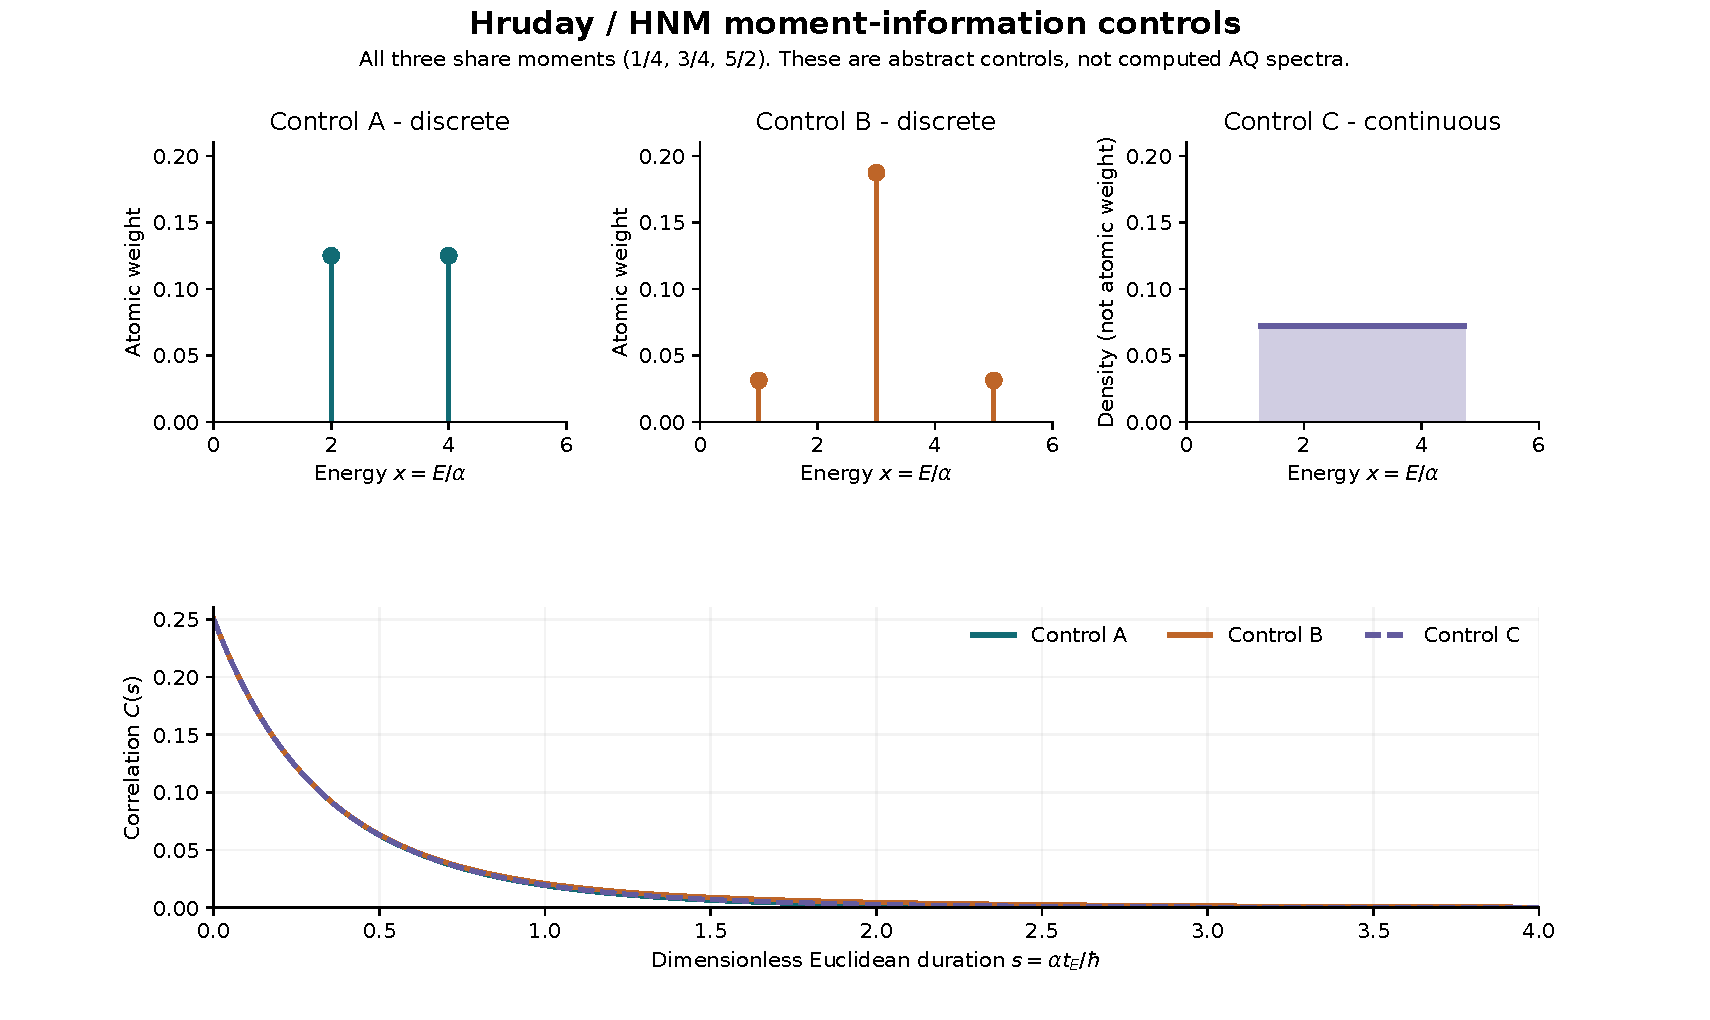
\includegraphics[width=\textwidth,height=.78\textheight,keepaspectratio]{figures/hnm-spectral-certificates.pdf}

\caption{Three positive spectral measures share the same zeroth, first and second moments but differ in atomic structure and Euclidean correlations. A and B are the exact discrete controls; C is the uniform density on [3-sqrt(3),3+sqrt(3)] with total mass1/4. Density and atomic-weight axes are distinguished. These are information-limit controls, not spectra computed for the AQ lattice Hamiltonian. Floating-point renderings of exact analytic formulas; the proof and rational inverse-moment enclosures are in AT2.}\label{fig:r30-at2}

\end{figure}\clearpage

\clearpage\hypertarget{r30-at2-forward-hruday-spectral-window-and-inverse-energy-certificate-at2-forward}{%
\section{Hruday AT2: spectral-window and inverse-energy certificate (forward derivation)}\label{r30:at2:forward:r30-at2-forward-hruday-spectral-window-and-inverse-energy-certificate-at2-forward}}

\begin{quote}\small\textbf{Source-bound forward derivation.} This is the complete typeset mathematical report of one producer. Prospective claims describe its original freeze; the shared reviewed result and permitted refinements are stated in the admission section. The two agents share inherited premises and model ancestry. This is neither an independent physical observation nor external human peer review.\end{quote}
Human project author: \textbf{Hruday N M (BUNZEEY)}. AI-assisted forward derivation independently executed before reading any current AT2 reverse or skeptic solution. HNM tags are project aliases, not claims to have invented moment duality, Jensen/Cauchy inequalities or reciprocal polynomial identities. Model-specific application; scientific priority is unverified.

\textbf{Result in the actual AQ state.} The original centered Wilson spectral measure satisfies

\begin{equation}
\hnmfit{\nu([\alpha/16,8\alpha])\ge\frac{307992}{1984375},\qquad
\frac{3843876001}{47000000000\alpha}
\le\langle\chi,H_{phys}^{-1}\chi\rangle
\le\frac{28462237549}{7503125000\alpha}.}
\tag{HNM-AT2-F01}\label{r30:at2:forward:eq1}
\end{equation}

The interval is a conservative certificate, not an optimal reconstruction. The lower inverse endpoint in (F01) uses the standard Cauchy baseline, which slightly improves the frozen c=3 tangent. None of these bounds identifies a particle pole or makes an infinite-volume susceptibility assertion.

\hypertarget{r30-at2-forward-exact-shared-state-normalization-and-uncertainty}{%
\subsection{Exact shared state, normalization and uncertainty}\label{r30:at2:forward:r30-at2-forward-exact-shared-state-normalization-and-uncertainty}}

Take exactly the AQ numerical-cap state and physical reducing generator admitted in AQ2 and AT1, with the original centered Wilson vector chi. The inherited gap is \(H_{\mathrm{phys}}\ge \alpha/16\) on the vacuum-orthogonal sector, and chi belongs to that sector. Define the dimensionless pushforward \(\eta(B)=\nu(\alpha B)\), \(x=E/\alpha\), \(a=1/16\). With \(w=\omega_{\mathrm{num}}(W)\), \(q=\omega_{\mathrm{num}}(W^{2})\), put

\begin{equation}
\hnmfit{\begin{gathered}
s=\int d\eta=q-w^2,\quad u=\int x\,d\eta=1-q,
\\
v=\int x^2d\eta\le B=36+98|\tau|,
\quad \operatorname{supp}\eta\subseteq[a,\infty).
\end{gathered}}
\tag{HNM-AT2-F02}\label{r30:at2:forward:eq2}
\end{equation}

These are actual AQ moments. The second moment is bounded, not evaluated. AQ2's trace-norm estimate on the actual 48-link cover gives \(|w|\le 1/500\), \(|q-1/4|\le 1/500\). Write \(z=w^{2}\); the joint declared domain is

\begin{equation}
\hnmfit{\begin{gathered}
q_-:=31/125\le q\le63/250=:q_+,\quad 0\le z\le1/250000=:z_+,
\\
s=q-z\ge61999/250000,
\quad 187/250\le u\le94/125.
\end{gathered}}
\tag{HNM-AT2-F03}\label{r30:at2:forward:eq3}
\end{equation}

Actual q and w are not replaced by Haar values. In particular s and u share q and must be propagated jointly. The rectangular q,z enclosure may include more points than the actual Hamiltonian realizes; bounds valid throughout it are conservative for the actual state. It is deterministic analytic uncertainty, not a sampling covariance.

The frozen L=8, c=3 and b=49 are dimensionless certificate choices; they change neither state nor Hamiltonian. Positive alpha,hbar,E\_star and lattice spacing remain fixed. No AO/AQ state identification or continuum limit is used.

\hypertarget{r30-at2-forward-full-half-line-window-minorant}{%
\subsection{Full-half-line window minorant}\label{r30:at2:forward:r30-at2-forward-full-half-line-window-minorant}}

For any L\textgreater a and x\textgreater=a, the affine function \(p_L(x)=(L-x)/(L-a)\) obeys

\begin{equation}
\hnmfit{\frac{L-x}{L-a}\le\mathbf1_{[a,L]}(x).}
\tag{HNM-AT2-F04}\label{r30:at2:forward:eq4}
\end{equation}

For a\textless=x\textless=L its value lies between zero and one. For x\textgreater L it is negative while the indicator is zero. At x=L the minorant equals zero and the closed-window indicator equals one. Thus a possible atom at L is retained and never erroneously subtracted. Integrating this pointwise inequality is justified because eta has finite first moment. For L=8,

\begin{equation}
\hnmfit{\eta([a,8])\ge\frac{8s-u}{8-a}
=\frac{9q-8z-1}{127/16}
\ge\frac{307992}{1984375}.}
\tag{HNM-AT2-F05}\label{r30:at2:forward:eq5}
\end{equation}

The last expression increases with q and decreases with z, so its minimum over (F03) is exactly at q=q\_-, z=z\_+. This certificate uses the mass, first moment and support bound only; it does not use v or B. It proves at least this much unnormalized spectral weight in the window. It is not a hard upper spectral cutoff, a probability of one, or an assertion that the true spectrum ends at 8alpha.

\hypertarget{r30-at2-forward-meaning-and-units-of-the-inverse-energy-form}{%
\subsection{Meaning and units of the inverse-energy form}\label{r30:at2:forward:r30-at2-forward-meaning-and-units-of-the-inverse-energy-form}}

The physical vacuum-orthogonal subspace reduces the self-adjoint H\_phys and its spectrum there lies in \([\alpha/16,\infty)\). The spectral reciprocal on that subspace is a bounded positive operator with norm at most 16/alpha. Since chi is centered, its quadratic form is well-defined:

\begin{equation}
\hnmfit{R:=\langle\chi,(H_{phys}|_{\Omega^\perp})^{-1}\chi\rangle
=\int E^{-1}d\nu(E)=\alpha^{-1}I,
\quad I:=\int x^{-1}d\eta(x).}
\tag{HNM-AT2-F06}\label{r30:at2:forward:eq6}
\end{equation}

One may extend the inverse by zero on the vacuum, but not call it an inverse of the full operator at zero. R has inverse-energy units. Hbar is absent from an energy inverse; a frequency inverse would carry a different factor. This is a mathematically defined inverse-energy quadratic form. Identifying 2R with a derivative of a thermodynamic ground-state expectation would require a separately specified deformation, existence and differentiability of its state branch, and an interchange of thermodynamic/differentiation limits. None is assumed here, so no static-susceptibility assertion is made.

\hypertarget{r30-at2-forward-frozen-tangent-lower-certificate}{%
\subsection{Frozen tangent lower certificate}\label{r30:at2:forward:r30-at2-forward-frozen-tangent-lower-certificate}}

For any c\textgreater0 and x\textgreater0,

\begin{equation}
\hnmfit{\frac1x-\left(\frac2c-\frac{x}{c^2}\right)
=\frac{(x-c)^2}{c^2x}\ge0.}
\tag{HNM-AT2-F07}\label{r30:at2:forward:eq7}
\end{equation}

The denominator is strictly positive throughout the support. This is an algebraic identity and a whole-half-line proof, not a positivity grid. With c=3, integration and joint uncertainty propagation give

\begin{equation}
\hnmfit{I\ge\frac23s-\frac19u
=\frac{7q-6z-1}{9}
\ge\frac{91997}{1125000}.}
\tag{HNM-AT2-F08}\label{r30:at2:forward:eq8}
\end{equation}

Again the minimum is at q\_-,z\_+. No second-moment value is used. The tangent may be negative for large x; that does not spoil a lower bound.

\hypertarget{r30-at2-forward-frozen-quadratic-upper-certificate-and-correct-moment-sign}{%
\subsection{Frozen quadratic upper certificate and correct moment sign}\label{r30:at2:forward:r30-at2-forward-frozen-quadratic-upper-certificate-and-correct-moment-sign}}

For a\textgreater0, b\textgreater=a and x\textgreater=a, define the quadratic numerator N\_b(x)=\(x^{2}-(2b+a)x+b^{2}+2ab\). Direct polynomial expansion gives

\begin{equation}
\hnmfit{\frac{N_b(x)}{ab^2}-\frac1x
=\frac{(x-a)(x-b)^2}{ab^2x}\ge0.}
\tag{HNM-AT2-F09}\label{r30:at2:forward:eq9}
\end{equation}

The denominator is strictly positive, the first factor is nonnegative, and the last factor is a square. This proves the upper bound at every continuous x\textgreater=a, including x=a,b and the infinite tail. Integrating and using the \textbf{positive} x\^{}2 coefficient gives

\begin{equation}
\hnmfit{I\le\frac{v-(2b+a)u+(b^2+2ab)s}{ab^2}
\le\frac{B-(2b+a)(1-q)+(b^2+2ab)(q-z)}{ab^2}.}
\tag{HNM-AT2-F10}\label{r30:at2:forward:eq10}
\end{equation}

The replacement v\textless=B has the required direction only because \(1/(ab^{2})>0\). It is not an equality claim. For b=49, the numerator increases with B and q and decreases with z. Hence use \texttt{B\_cap=1800000049/50000000}, q=q\_+, z=0, obtaining

\begin{equation}
\hnmfit{I\le\frac{28462237549}{7503125000}.}
\tag{HNM-AT2-F11}\label{r30:at2:forward:eq11}
\end{equation}

The declared q,w relation remains intact during this calculation. These coefficients were frozen before execution; there is no tuning on outputs or claim that b=49 is optimal.

\hypertarget{r30-at2-forward-baseline-comparisons}{%
\subsection{Baseline comparisons}\label{r30:at2:forward:r30-at2-forward-baseline-comparisons}}

Cauchy-Schwarz applied to sqrt(x) and 1/sqrt(x) in L\^{}2(eta), and the support reciprocal bound, give

\begin{equation}
\hnmfit{\frac{s^2}{u}\le I\le\frac{s}{a}.}
\tag{HNM-AT2-F12}\label{r30:at2:forward:eq12}
\end{equation}

Both integrals needed for Cauchy are finite; u\textgreater0 follows explicitly from (F03). The function \((q-z)^{2}/(1-q)\) decreases with z and increases with q throughout the declared domain: its q derivative is \(2(q-z)/(1-q)+(q-z)^{2}/(1-q)^{2}>0\). Therefore the uniform Cauchy baseline is

\begin{equation}
\hnmfit{I\ge\frac{(61999/250000)^2}{94/125}
=\frac{3843876001}{47000000000}
>\frac{91997}{1125000},\qquad
I\le16q_+=\frac{504}{125}.}
\tag{HNM-AT2-F13}\label{r30:at2:forward:eq13}
\end{equation}

The frozen quadratic upper bound is strictly smaller than 504/125. Combining the stronger of the two valid lower bounds with the stronger upper bound produces (F01). All numbers are exact rationals. No strong-duality theorem, extremizer existence or global optimality is asserted.

\hypertarget{r30-at2-forward-equal-moments-do-not-identify-an-energy-atom}{%
\subsection{Equal moments do not identify an energy atom}\label{r30:at2:forward:r30-at2-forward-equal-moments-do-not-identify-an-energy-atom}}

The prescribed abstract controls are

\begin{equation}
\hnmfit{\eta_A=\frac{\delta_2+\delta_4}{8},\quad
\eta_B=\frac{\delta_1}{32}+\frac{3\delta_3}{16}+\frac{\delta_5}{32},\quad
\eta_C=\tfrac14\operatorname{Uniform}[3-\sqrt3,3+\sqrt3].}
\tag{HNM-AT2-F14}\label{r30:at2:forward:eq14}
\end{equation}

For A and B, direct finite sums give \((s,u,v)=(1/4,3/4,5/2)\). For C, write x=3+y with y uniformly distributed on \texttt{{[}-sqrt3,sqrt3{]}}. Symmetry gives E{[}y{]}=0, and elementary integration gives E{[}y\^{}2{]}=3/3=1. Multiplying the resulting moments 1,3,10 by 1/4 gives the same triple. The support of C lies strictly above one because sqrt3\textless2, hence all three supports are above a. All obey the moment relations at q=1/4,w=0 and satisfy v\textless=B. A and B have distinct atom sets; C has a bounded interval density and no atoms.

Their inverse moments are nevertheless different:

\begin{equation}
\hnmfit{I_A=\frac3{32},\qquad I_B=\frac1{10},\qquad
I_C=\frac{1}{8\sqrt3}\log\frac{3+\sqrt3}{3-\sqrt3}
=\frac1{12}\sum_{k=0}^{\infty}\frac{1}{3^k(2k+1)}.}
\tag{HNM-AT2-F15}\label{r30:at2:forward:eq15}
\end{equation}

The integral formula follows by integrating 1/x against the uniform density \texttt{1/(8sqrt3)}. The series follows from integrating the geometric series for \(1/(1-t^{2})\) from zero to 1/sqrt3, where it converges absolutely and uniformly on that closed interval. There is no uncontrolled logarithm evaluation. The first three terms are 17/180. For k\textgreater=3, \(1/(2k+1)\le 1/7\) and the geometric sum of 3\^{}-k is 1/18. Therefore

\begin{equation}
\hnmfit{\frac3{32}<\frac{17}{180}<I_C
\le\frac{17}{180}+\frac1{1512}
=\frac{719}{7560}<\frac1{10}.}
\tag{HNM-AT2-F16}\label{r30:at2:forward:eq16}
\end{equation}

Strictness on the lower side follows from the positive remaining series. Thus even exact knowledge of all three contracted moments, stronger than AT1's second-moment ceiling, does not determine spectral atom structure or inverse-energy response. Each fixture is realized abstractly by multiplication by x on L\^{}2(eta), with source vector 1; adding an orthogonal one-dimensional zero-energy vacuum realizes a centered nonnegative spectral problem. This is not a realization by the AQ lattice Hamiltonian. The controls establish insufficiency of the moment information, not actual thermodynamic-state nonuniqueness or multiple AQ phases.

\hypertarget{r30-at2-forward-controls-source-ancestry-and-scope}{%
\subsection{Controls, source ancestry and scope}\label{r30:at2:forward:r30-at2-forward-controls-source-ancestry-and-scope}}

The exact checker expands the rational identities as polynomial coefficient arrays, checks endpoint propagation with rational arithmetic, and integrates the finite and uniform moment fixtures symbolically. Whole-half-line validity comes from the factorization and sign proofs, not the diagnostic sample evaluations. A polynomial \((x-3/2)^{2}-1/16\) is positive at all integer sample nodes but negative at 3/2, exposing grid-only positivity. A negative-quadratic kernel control shows why replacing v by B in an upper bound with a negative coefficient is invalid. Further controls preserve an atom at x=8, distinguish a second-moment ceiling from equality, reject substituting q=1/4,w=0 for the allowed interacting unknowns, and verify the alpha\^{}-1 scaling.

Bertsimas and Popescu, \emph{SIAM J. Optim.} 15 (2005), Sections 2-3, supply classical ancestry for polynomial moment certificates and the upper-moment coefficient-sign rule. Abbott, Fields, Jay, Oare and Saccardi, arXiv:2605.20509v1, III.1, IV.1-IV.3 and VII.4, provide current spectral-kernel certificate context and explicitly distinguish extremal feasible spectra from the true spectrum. Selected passages and the panel's source record were consulted, not the entirety of either research program. The contribution here is this particular AQ dictionary, evaluated enclosure and exact controls; generic methods are not Hruday inventions.

Run {\small\path{python -B research/round30/forward/at2/check.py --output /absolute/new/directory}}. Normal and optimized results must match. The checker and report use only stdlib/exact arithmetic. No physical susceptibility, pole, exact mass, sharpness, state identification or continuum Yang-Mills result is claimed. Loop 3 awaits advisor selection after the separate skeptical review.

\repo{research/round30/forward/at2/report.md}


\clearpage\hypertarget{r30-at2-reverse-hruday-spectral-window-and-inverse-energy-certificate-reverse-at2}{%
\section{Hruday AT2: spectral-window and inverse-energy certificate (reverse derivation)}\label{r30:at2:reverse:r30-at2-reverse-hruday-spectral-window-and-inverse-energy-certificate-reverse-at2}}

\begin{quote}\small\textbf{Source-bound reverse derivation.} This is the complete typeset mathematical report of one producer. Prospective claims describe its original freeze; the shared reviewed result and permitted refinements are stated in the admission section. The two agents share inherited premises and model ancestry. This is neither an independent physical observation nor external human peer review.\end{quote}
Human author: \textbf{Hruday N M (BUNZEEY)}. AI-assisted independent reverse reconstruction; scientific priority unverified. HNM labels are traceable project aliases. No current forward or skeptic AT2 result was read. The shared prospective certificate choices and inherited admitted premises are disclosed and copied in {\small\path{inputs/}}.

\hypertarget{r30-at2-reverse-reverse-reconstruction-from-the-requested-observable}{%
\subsection{Reverse reconstruction from the requested observable}\label{r30:at2:reverse:r30-at2-reverse-reverse-reconstruction-from-the-requested-observable}}

The two target functionals are the mass of a fixed finite energy interval and the inverse-energy quadratic form. They are integrals against the same positive spectral measure. A complete pointwise minorant/majorant on its entire support therefore suffices. Only a second-moment upper bound is available, so the quadratic coefficient's sign must permit replacing that moment by its ceiling. This reverse argument determines the proof obligations before numerical evaluation. It does not reconstruct a unique spectrum from moments.

Use exactly AQ's chosen state and original centered Wilson vector, now with AT1's operator-domain and first-moment identity. Let eta be the pushforward of its positive spectral measure under x=E/alpha. Define

\begin{equation}
\hnmfit{\begin{gathered}
a=\frac1{16},\quad w=\omega_{num}(W),\\
q=\omega_{num}(W^2),\quad s=\int d\eta=q-w^2,\\
u=\int x\,d\eta=1-q,\quad v=\int x^2d\eta\le B=36+98|\tau|.
\end{gathered}}
\tag{HNM-AT2-R01}\label{r30:at2:reverse:eq1}
\end{equation}

The support is contained in {[}a,infinity). AQ2 and \textbar tau\textbar\textless=10\^{}-8 provide the convenient weak rational bounds

\begin{equation}
\hnmfit{q_-:=\frac{31}{125}\le q\le q_+:=\frac{63}{250},\quad
 0\le z:=w^2\le z_+:=\frac1{250000},\quad
 B\le B_*:=\frac{1800000049}{50000000}.}
\tag{HNM-AT2-R02}\label{r30:at2:reverse:eq2}
\end{equation}

These follow because 2sqrt(98\textbar tau\textbar)\textless1/500. The q,w uncertainty is deterministic analytic uncertainty, not sampled statistical error. We retain the joint relations s=q-z and u=1-q; independent optimization of unrelated moment intervals is not claimed. The rectangular q,z enclosure can contain points not realized by the actual model. Monotone endpoint substitution below gives valid uniform bounds, without asserting sharpness over its actual realizable states.

The frozen choices L=8,c=3,b=49 are dimensionless certificate parameters. They are not Hamiltonian couplings, regulators, fitted energies or predictions of pole locations. Alpha,hbar,spacing and E\_star remain fixed positive.

\hypertarget{r30-at2-reverse-a-closed-finite-spectral-window}{%
\subsection{A closed finite spectral window}\label{r30:at2:reverse:r30-at2-reverse-a-closed-finite-spectral-window}}

For x\textgreater=a the affine function p\_L(x)=(L-x)/(L-a) is at most one on {[}a,L{]}, and is negative above L. Since L\textgreater a, this proves on the whole half-line

\begin{equation}
\hnmfit{\frac{L-x}{L-a}\le\mathbf1_{[a,L]}(x),\qquad
 \eta([a,L])\ge\frac{Ls-u}{L-a}
 =\frac{(L+1)q-Lz-1}{L-a}.}
\tag{HNM-AT2-R03}\label{r30:at2:reverse:eq3}
\end{equation}

At x=L the minorant is zero but the indicator is one. A possible endpoint atom is therefore retained rather than silently discarded. Finite first moment makes the affine function integrable even though it becomes negative without bound at large x.

The last expression increases with q and decreases with z. Insert q\_-,z\_+ and L=8 to obtain the exact Hruday window certificate

\begin{equation}
\hnmfit{\boxed{\nu([\alpha/16,8\alpha])=\eta([1/16,8])
 \ge\frac{307992}{1984375}>\frac{31}{200}.}}
\tag{HNM-AT2-R04}\label{r30:at2:reverse:eq4}
\end{equation}

The floor is approximately 0.15520857 of the unnormalized Wilson spectral weight. It is a mass guarantee, not a statement that all weight lies below 8alpha. This bound uses the gap and first moment, not the second-moment ceiling.

\hypertarget{r30-at2-reverse-inverse-on-the-actual-physical-subspace-and-units}{%
\subsection{Inverse on the actual physical subspace and units}\label{r30:at2:reverse:r30-at2-reverse-inverse-on-the-actual-physical-subspace-and-units}}

AQ2 makes the physical vacuum-orthogonal subspace reducing, and H restricted to it obeys H\textgreater=alpha a. Functional calculus thus defines a bounded positive inverse on the whole subspace, with norm at most 1/(alpha a), and also a bounded inverse square root. Since chi is centered, it lies in that subspace. Therefore

\begin{equation}
\hnmfit{R:=\langle\chi,H^{-1}\chi\rangle
 =\|H^{-1/2}\chi\|^2
 =\frac1\alpha\int_a^\infty\frac1x\,d\eta(x),\qquad
 0\le R\le\frac{s}{\alpha a}.}
\tag{HNM-AT2-R05}\label{r30:at2:reverse:eq5}
\end{equation}

The inverse is not defined by inverting the vacuum eigenvalue zero. It is the reduced inverse (or equivalently the bounded pseudoinverse set to zero on the vacuum). R has units inverse energy; alpha R is dimensionless. The inverse of the frequency generator H/hbar instead gives hbar R. No differentiability of a deformed infinite-volume ground state, or static susceptibility, follows from this functional calculus alone.

\hypertarget{r30-at2-reverse-entire-half-line-reciprocal-certificates}{%
\subsection{Entire-half-line reciprocal certificates}\label{r30:at2:reverse:r30-at2-reverse-entire-half-line-reciprocal-certificates}}

For every x\textgreater0, the tangent at c\textgreater0 has the exact positive residual

\begin{equation}
\hnmfit{\ell_c(x)=\frac2c-\frac{x}{c^2},\qquad
 \frac1x-\ell_c(x)=\frac{(x-c)^2}{c^2x}\ge0.}
\tag{HNM-AT2-R06}\label{r30:at2:reverse:eq6}
\end{equation}

For every x\textgreater=a\textgreater0 and b\textgreater=a the proposed quadratic satisfies

\begin{equation}
\hnmfit{P_b(x)=\frac{x^2-(2b+a)x+b^2+2ab}{ab^2},\qquad
 P_b(x)-\frac1x=\frac{(x-a)(x-b)^2}{ab^2x}\ge0.}
\tag{HNM-AT2-R07}\label{r30:at2:reverse:eq7}
\end{equation}

The denominators are strictly positive throughout the support. These factorizations prove global half-line domination, including arbitrarily large energies; a numerical grid is unnecessary. Integrating positive inequalities is weak duality. No strong duality or optimality theorem is used.

The coefficient of x\^{}2 in P\_b is +1/(ab\^{}2)\textgreater0. Consequently v\textless=B may be substituted in the upper-bound direction. A negative coefficient would reverse that substitution inequality. The tangent has zero quadratic coefficient and uses no second-moment information. With c=3,b=49, let A=2b+a and D=b\^{}2+2ab. Then

\begin{equation}
\hnmfit{\frac{7q-6z-1}{9}
 \le\alpha R
 \le\frac{B-A+(A+D)q-Dz}{ab^2}.}
\tag{HNM-AT2-R08}\label{r30:at2:reverse:eq8}
\end{equation}

Here A,D,A+D and ab\^{}2 are positive. The lower expression is smallest at q\_-,z\_+; the upper expression is largest in this enclosure at B\_*,q\_+,z=0. Exact rational arithmetic gives

\begin{equation}
\hnmfit{\boxed{\frac{91997}{1125000}\le\alpha R
 \le\frac{28462237549}{7503125000}.}}
\tag{HNM-AT2-R09}\label{r30:at2:reverse:eq9}
\end{equation}

These are approximately 0.08177511 and 3.79338443. The second moment remains an upper bound throughout; no value v=B is assigned to the actual AQ measure.

\hypertarget{r30-at2-reverse-preserve-and-compare-the-elementary-baselines}{%
\subsection{Preserve and compare the elementary baselines}\label{r30:at2:reverse:r30-at2-reverse-preserve-and-compare-the-elementary-baselines}}

Cauchy--Schwarz applied to sqrt(x) and 1/sqrt(x) in L2(eta) yields s\^{}2\textless=u integral x\^{}-1 d eta. Both functions are square integrable: u is finite by AT1, and inverse integrability follows from a\textgreater0. Also u=1-q\textgreater=1-q\_+\textgreater0. The support bound remains as in (R05):

\begin{equation}
\hnmfit{\frac{s^2}{u}\le\alpha R\le\frac{s}{a}.}
\tag{HNM-AT2-R10}\label{r30:at2:reverse:eq10}
\end{equation}

The lower expression (q-z)\^{}2/(1-q) decreases with z, because q-z\textgreater0. Its q derivative is (q-z)(2-q-z)/(1-q)\^{}2\textgreater0 throughout the declared box. Thus its uniform floor is attained at q\_-,z\_+ within that box. The upper support ceiling is at q\_+,z=0. Therefore

\begin{equation}
\hnmfit{\frac{3843876001}{47000000000}\le\alpha R\le\frac{504}{125}.}
\tag{HNM-AT2-R11}\label{r30:at2:reverse:eq11}
\end{equation}

The Cauchy floor is slightly stronger than the frozen c=3 tangent, while the polynomial upper bound is stronger than the support ceiling. The certificate package consequently permits the combined interval

\begin{equation}
\hnmfit{\boxed{\frac{3843876001}{47000000000\,\alpha}\le R
 \le\frac{28462237549}{7503125000\,\alpha}.}}
\tag{HNM-AT2-R12}\label{r30:at2:reverse:eq12}
\end{equation}

Its lower endpoint is approximately 0.08178460/alpha. The tangent remains recorded as a independently checked frozen certificate, with its honest baseline comparison. No parameter was retuned to hide this comparison, and no globally optimal interval is claimed.

\hypertarget{r30-at2-reverse-equal-moments-do-not-specify-spectral-type-or-inverse-energy}{%
\subsection{Equal moments do not specify spectral type or inverse energy}\label{r30:at2:reverse:r30-at2-reverse-equal-moments-do-not-specify-spectral-type-or-inverse-energy}}

Consider the following abstract dimensionless positive measures, solely as information-content controls:

\begin{equation}
\hnmfit{\eta_A=\frac{\delta_2+\delta_4}{8},\quad
 \eta_B=\frac{\delta_1}{32}+\frac{3\delta_3}{16}+\frac{\delta_5}{32},\quad
 \eta_C=\frac14\operatorname{Uniform}[3-\sqrt3,3+\sqrt3].}
\tag{HNM-AT2-R13}\label{r30:at2:reverse:eq13}
\end{equation}

Their supports lie above a: 3-sqrt3\textgreater1\textgreater a because sqrt3\textless2. A and B have different finite atom sets. C has a bounded Lebesgue density on its interval and no atoms. Direct sums give the first three moments of A and B. For C, write X=3+Y with Y uniform on {[}-sqrt3,sqrt3{]}. Symmetry gives E Y=0 and E Y\textsuperscript{2=(sqrt3)}2/3=1. Hence all three have

\begin{equation}
\hnmfit{(\int d\eta,\int x\,d\eta,\int x^2d\eta)
 =\left(\frac14,\frac34,\frac52\right).}
\tag{HNM-AT2-R14}\label{r30:at2:reverse:eq14}
\end{equation}

These match the contracted relation at q=1/4,w=0 and lie strictly below B even at tau=0. They show insufficiency even if the second moment were supplied exactly, more information than the actual AT1 ceiling.

Their inverse moments are

\begin{equation}
\hnmfit{r_A=\frac3{32},\quad r_B=\frac1{10},\quad
 r_C=\frac1{8\sqrt3}\log\frac{3+\sqrt3}{3-\sqrt3}
 =\frac1{12}\sum_{k=0}^\infty\frac{3^{-k}}{2k+1}.}
\tag{HNM-AT2-R15}\label{r30:at2:reverse:eq15}
\end{equation}

For the series identity, expand 1/(3+Y) in its uniformly convergent geometric series on \textbar Y\textbar\textless=sqrt3\textless3 and integrate: odd powers vanish and the even uniform moments are 3\^{}k/(2k+1). The exact remainder after terms k=0,\ldots,N-1 is positive and bounded by

\begin{equation}
\hnmfit{0<r_C-\frac1{12}\sum_{k=0}^{N-1}\frac{3^{-k}}{2k+1}
 \le\frac{3^{-N}}{8(2N+1)}.}
\tag{HNM-AT2-R16}\label{r30:at2:reverse:eq16}
\end{equation}

At N=8 the rational enclosure is

\begin{equation}
\hnmfit{\frac3{32}<\frac{1872586}{19702683}<r_C
 \le\frac{254674699}{2679564888}<\frac1{10}.}
\tag{HNM-AT2-R17}\label{r30:at2:reverse:eq17}
\end{equation}

Thus identical zeroth, first and second moments permit different inverse responses, and an atomic or atomless measure. Each fixture has an abstract self-adjoint multiplication realization on L2(eta), source vector 1, and an added vacuum summand. This construction does not realize the actual AQ Hamiltonian. It proves neither multiple AQ thermodynamic states nor any claim about which spectral type AQ actually possesses. In particular moments alone do not identify a particle pole, an exact mass, or b=49 as an energy atom.

\hypertarget{r30-at2-reverse-exact-controls-and-provenance}{%
\subsection{Exact controls and provenance}\label{r30:at2:reverse:r30-at2-reverse-exact-controls-and-provenance}}

The standard-library checker verifies polynomial coefficient identities, all rational endpoints, monotonicity coefficient signs and all equal-moment arithmetic. Its executed controls include:

\begin{itemize}
\tightlist
\item
  A negative quadratic coefficient with v\textless B reverses the putative upper-bound substitution. In contrast the actual P\_b coefficient is positive, and the strict substitution slack is computed on eta\_A.
\item
  The polynomial (x-3/2)\^{}2-1/16 is positive at the frozen sampled points a,1,2,3,8,49,100, but negative at x=3/2. This rejects a sampled-grid certificate. The actual certificates use exact factorizations instead.
\item
  A permitted joint moment point q=q\_-,w=1/500 has s and u different from the Haar values. A one-atom abstract measure of mass s at u/s realizes those moments with v=u\^{}2/s\textless B. It invalidates an assignment of Haar values to unknown interacting moments; it does not claim every Haar-substituted numerical bound happens to fail.
\item
  The endpoint atom delta\_L has window mass one while p\_L(L)=0. A separate measure with positive high-energy weight above L verifies that a mass floor is not a hard spectral cutoff.
\item
  A/B/C have exactly equal moments and different inverse responses, including atomless C. The v ceiling is strictly larger than their exact second moments.
\item
  Rescaling alpha changes R inversely, and replacing energy by frequency introduces hbar. Dimensionless inverse integrals cannot be presented as an energy inverse unchanged.
\item
  In a two-state diagnostic H=diag(0,3), W=sigma\_x/2, R=1/12. Perturbations H-fW and H-2fW have different derivatives of the W expectation, 2R and 4R, despite identical undeformed R. This demonstrates the missing source-calibration requirement. Even after fixing a source, existence and interchange of derivatives for an infinite-volume deformed AQ state remain unproved; this finite fixture does not establish that differentiability.
\end{itemize}

Bertsimas and Popescu, \emph{SIAM J. Optim.} 15 (2005), Sections 2--3, provide the moment-duality and polynomial-positivity ancestry, including the upper-moment coefficient-sign condition. Abbott et al., arXiv:2605.20509v1, Sections III.1, IV.1--IV.3 and VII.4, give the current spectral-kernel certificate context and caution about interpreting extremal feasible measures as the true spectrum. Those primary passages were checked with the source panel and direct reading. Their general methods retain attribution. The Hruday/HNM contribution is this model-specific AQ application, exact physical interval and discriminating countercontrols; priority is unverified.

Reproduce with {\small\path{python -B research/round30/reverse/at2/check.py --output /absolute/fresh-directory}}. Every source, report, checker and output is hash-bound; normal and optimized Python output bytes are compared. Finite controls audit algebra and counter-inferences; the full-half-line proofs above establish certificate validity. No global optimization, actual susceptibility, unique spectrum or continuum conclusion is asserted. AT2 ends here; Loop 3 remains unselected pending its review.

\repo{research/round30/reverse/at2/report.md}


\clearpage\section{Hruday AT3: reviewed admission}

\label{stmt:AT3}

\textbf{Verdict: accepted within scope.} The fixed 4097-node protocol conditionally encloses $I=\alpha R$ when supplied certified centered AQ samples with absolute error at most $10^{-6}$. Exact rational data give interval width below $1/500$; arithmetic bins contribute their explicitly bounded trapezoid width. Both executed abstract A/B benchmarks pass, and their full admissible-error output envelopes are disjoint. No actual AQ correlation samples or response value are supplied.

\subsection*{Limits and independent review}

The producer reports were frozen separately before exchange. Their common ancestry, contract and inherited methods remain disclosed. The skeptic reviewed both proofs and executed controls; this does not constitute external human peer review.

\begin{itemize}

\item No actual AQ correlation samples or inverse response evaluated

\item Forward permits arbitrary arithmetic bins and reports width verdict; reverse admits bins \(\le 1e-12\) and guarantees the width target

\item Input validation does not certify centering, model/state provenance or scientific error bounds

\item A/B and the separately disclosed damaging tail control are abstract measures, not AQ simulations

\item No susceptibility, identified pole, optimal design, state uniqueness or continuum construction

\item Scientific priority unverified; established methods retain attribution

\item Exactly three investigations; no fourth scientific execution

\end{itemize}

\repo{research/round30/advisor/at3-gate.json}

\par\repo{research/round30/skeptic/at3.md}

\subsection*{Substantive directional differences}

\begin{itemize}

\item Forward uses degree39/40 and reverse degree33/32 alternating exponential brackets; both enclose every node using outward rational arithmetic.

\item Forward accepts arbitrary arithmetic bins and reports a width verdict; reverse requires bins no wider than10\textasciicircum{}-12 to guarantee the target.

\item The reverse omitted-tail diagnostic internally evaluates a third abstract curve; this is required countercontrol work, not an additional investigation or AQ simulation.

\end{itemize}

\subsection*{The two reusable input domains}

The forward \repo{evaluator.py} accepts exact rational sample values or enclosing pairs. Wider arithmetic bins still yield a conditional enclosing interval, but can fail its width verdict. The reverse \repo{check.py} evaluator requires enclosing pairs, arithmetic width at most $10^{-12}$, and its additional mass/error envelope checks; its CSV route also validates the complete time grid. These are different admitted API domains, not interchangeable promises.

For both APIs, callers must establish centering, the actual AQ state/model provenance and the deterministic sample-error premise. Syntax checks cannot certify those physical conditions. The executed CSV data are synthetic A/B controls, and no actual AQ correlation samples or response value are supplied.

\clearpage\begin{figure}[p]\centering

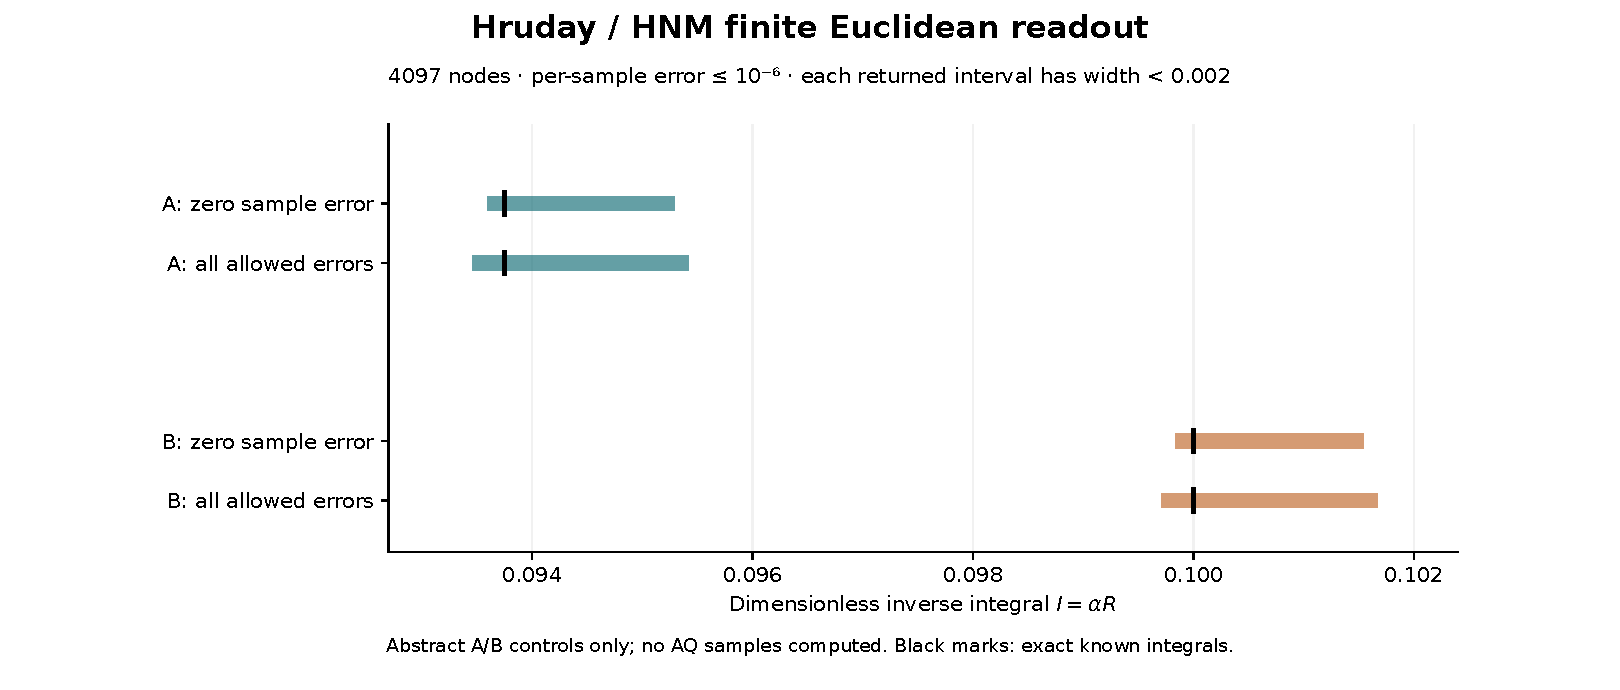
\includegraphics[width=\textwidth,height=.78\textheight,keepaspectratio]{figures/hnm-euclidean-readout.pdf}

\caption{Certified inverse-integral intervals for the two abstract equal-moment controls A and B. The zero-error rows still include the protocol error allowances. The all-errors rows are envelopes of possible returned intervals: they include both the observed-sum shift and the sample allowance inside each certificate. Each individual returned interval has width below 0.002; its full varying-data envelope can be wider. The envelopes remain separated by more than 0.004293. Black marks show the known exact values 3/32 and 1/10. These are synthetic controls, not AQ measurements or computed AQ response values. Floating-point rendering of frozen exact rational endpoints; the source output supplies rigorous enclosures.}\label{fig:r30-at3}

\end{figure}\clearpage

\clearpage\hypertarget{r30-at3-forward-hruday-finite-euclidean-readout-certificate-at3-forward}{%
\section{Hruday AT3: finite Euclidean readout certificate (forward derivation)}\label{r30:at3:forward:r30-at3-forward-hruday-finite-euclidean-readout-certificate-at3-forward}}

\begin{quote}\small\textbf{Source-bound forward derivation.} This is the complete typeset mathematical report of one producer. Prospective claims describe its original freeze; the shared reviewed result and permitted refinements are stated in the admission section. The two agents share inherited premises and model ancestry. This is neither an independent physical observation nor external human peer review.\end{quote}
Human project author: \textbf{Hruday N M (BUNZEEY)}. AI-assisted independent forward execution, without reading current AT3 reverse or skeptic solutions. HNM tags are project aliases for this application of established quadrature and spectral methods. Scientific priority is unverified.

\textbf{Outcome:} the frozen design certifies a conditional AQ inverse-form readout with interval width below 1/500 for exact rational reported data meeting its error contract. Its two executed abstract fixtures pass, including all-positive/all-negative sample errors; their worst-case output envelopes are disjoint. \textbf{No actual AQ correlation samples or actual AQ inverse value have been produced.}

\hypertarget{r30-at3-forward-actual-state-conditional-theorem-and-physical-clock}{%
\subsection{Actual-state conditional theorem and physical clock}\label{r30:at3:forward:r30-at3-forward-actual-state-conditional-theorem-and-physical-clock}}

Use exactly AT1/AT2's actual AQ centered Wilson spectral measure eta in dimensionless energy x=E/alpha. Its inherited hypotheses are support x\textgreater=a=1/16, mass \(m\le M=63/250\), first moment \(u\le U=94/125\), and finite second moment \(v\le B=36+98|\tau|\). To avoid confusing Euclidean duration with mass, denote mass by m in this report and duration by s. Define

\begin{equation}
\hnmfit{C(s)=\int e^{-sx}\,d\eta(x),\qquad
I=\int_0^\infty C(s)\,ds=\int x^{-1}d\eta(x)=\alpha R.}
\tag{HNM-AT3-F01}\label{r30:at3:forward:eq1}
\end{equation}

Positivity permits Tonelli, and x\textgreater=a\textgreater0 gives I\textless=M/a\textless infinity. Here R is precisely AT2's reduced inverse-energy quadratic form, not a thermodynamic susceptibility. In physical Euclidean time,

\begin{equation}
\hnmfit{s=\alpha t_E/\hbar,\quad C_{phys}(t_E)=C(\alpha t_E/\hbar),\quad
R=\hbar^{-1}\int_0^\infty C_{phys}(t_E)\,dt_E.}
\tag{HNM-AT3-F02}\label{r30:at3:forward:eq2}
\end{equation}

The frozen design is

\begin{equation}
\hnmfit{T=128,\quad h=1/32,\quad N=4096,\quad Nh=T,\quad
\epsilon=10^{-6},\quad N+1=4097.}
\tag{HNM-AT3-F03}\label{r30:at3:forward:eq3}
\end{equation}

Thus the physical endpoint is \(128 \hbar/\alpha\) and the physical sample spacing is \(\hbar/(32\alpha)\). Sample errors are deterministic absolute errors on dimensionless C(s), not Gaussian noise, independent random errors or confidence intervals. This protocol supplies no claim that obtaining those data is experimentally or computationally feasible.

\hypertarget{r30-at3-forward-differentiability-and-integrated-curvature-from-actual-moments}{%
\subsection{Differentiability and integrated curvature from actual moments}\label{r30:at3:forward:r30-at3-forward-differentiability-and-integrated-curvature-from-actual-moments}}

Since m,u,v are finite, dominated convergence on each compact nonnegative duration interval yields right derivatives at zero and ordinary derivatives thereafter:

\begin{equation}
\hnmfit{C'(s)=-\int x e^{-sx}d\eta(x),\qquad
C''(s)=\int x^2e^{-sx}d\eta(x)\ge0.}
\tag{HNM-AT3-F04}\label{r30:at3:forward:eq4}
\end{equation}

Continuity of C'\,' at zero follows from domination by the integrable x\^{}2. There is no third-moment assumption. More usefully than a pointwise supremum, Tonelli gives

\begin{equation}
\hnmfit{\int_0^T C''(s)\,ds=\int x(1-e^{-Tx})d\eta(x)\le u\le U.}
\tag{HNM-AT3-F05}\label{r30:at3:forward:eq5}
\end{equation}

Only nonnegative integrands are interchanged. The second moment justifies C\^{}2 regularity; the final quadrature constant uses the smaller integrated first moment U.

\hypertarget{r30-at3-forward-exact-peano-identity-and-quadrature-sign}{%
\subsection{Exact Peano identity and quadrature sign}\label{r30:at3:forward:r30-at3-forward-exact-peano-identity-and-quadrature-sign}}

On cell \texttt{{[}jh,(j+1)h{]}}, take \(k_j(s)=(s-jh)((j+1)h-s)/2\). It vanishes at both endpoints, with derivatives h/2 and -h/2 there and second derivative -1. Two integrations by parts yield

\begin{equation}
\hnmfit{\frac h2[C(jh)+C((j+1)h)]-\int_{jh}^{(j+1)h}C(s)ds
=\int_{jh}^{(j+1)h}k_j(s)C''(s)ds.}
\tag{HNM-AT3-F06}\label{r30:at3:forward:eq6}
\end{equation}

The kernel satisfies \(0\le k_j\le h^{2}/8\) throughout the continuous cell. Summing and using (F05), with \texttt{Trap(C)=h(C(0)/2+sum\_(j=1)\^{}(N-1)\ C(jh)+C(T)/2)}, proves

\begin{equation}
\hnmfit{0\le\operatorname{Trap}(C)-\int_0^T C(s)ds
\le Q:=h^2U/8=47/512000.}
\tag{HNM-AT3-F07}\label{r30:at3:forward:eq7}
\end{equation}

The trapezoid rule overestimates the finite integral because C is convex. Treating Q as an amount to add to a lower endpoint gives the wrong sign. No observed mesh convergence or finite positivity grid supplies this theorem.

\hypertarget{r30-at3-forward-infinite-time-tail-and-deterministic-sample-budget}{%
\subsection{Infinite-time tail and deterministic sample budget}\label{r30:at3:forward:r30-at3-forward-infinite-time-tail-and-deterministic-sample-budget}}

Support above a gives

\begin{equation}
\hnmfit{0\le\int_T^\infty C(s)ds
=\int e^{-Tx}x^{-1}d\eta(x)
\le D:=\frac{M}{a}e^{-aT}=\frac{504}{125}e^{-8}.}
\tag{HNM-AT3-F08}\label{r30:at3:forward:eq8}
\end{equation}

For reported real samples y\_j satisfying \(|y_j-C(jh)|\le \epsilon\), all trapezoid weights are positive and sum hN=T. Therefore

\begin{equation}
\hnmfit{|\operatorname{Trap}(y)-\operatorname{Trap}(C)|\le T\epsilon
=2/15625=:J.}
\tag{HNM-AT3-F09}\label{r30:at3:forward:eq9}
\end{equation}

The vectors with every error +epsilon and every error -epsilon attain +J and -J. A root-N allowance would be invalid for this deterministic model. Combining (F07)-(F09) yields the conditional interval

\begin{equation}
\hnmfit{I\in[\operatorname{Trap}(y)-Q-J,\ \operatorname{Trap}(y)+D+J].}
\tag{HNM-AT3-F10}\label{r30:at3:forward:eq10}
\end{equation}

For arithmetic enclosures \(y_j in [l_j,r_j]\), use the corresponding positive-weight lower and upper sums P\_-,P\_+. With a proved rational upper D\_+ for D,

\begin{equation}
\hnmfit{I\in[P_--Q-J,\ P_++D_++J],\quad
\text{width}=(P_+-P_-)+Q+D_++2J.}
\tag{HNM-AT3-F11}\label{r30:at3:forward:eq11}
\end{equation}

The arithmetic width is separate from the physical/sample error budget. The API never treats unknown exponential roundoff as free. For exact rational y\_j the arithmetic width is zero. The certified error calculation gives \(Q+D_++2J<170039/100000000<1/500\). For the executed enclosures their extra width is below 10\^{}-24, so the frozen width target also passes.

\hypertarget{r30-at3-forward-directed-rational-exponential-arithmetic-and-complete-node-semantics}{%
\subsection{Directed rational exponential arithmetic and complete node semantics}\label{r30:at3:forward:r30-at3-forward-directed-rational-exponential-arithmetic-and-complete-node-semantics}}

The arithmetic scale \(G=10^{30}\) was fixed in evaluator.py before generating any fixture outcome. To enclose exp(-y) for rational y\textgreater=0, choose k so r=y/2\^{}k\textless=1/2. The alternating exponential Taylor terms decrease in absolute magnitude. Consequently the odd partial sum at degree39 and even partial sum at degree40 give

\begin{equation}
\hnmfit{\sum_{n=0}^{39}\frac{(-r)^n}{n!}
\le e^{-r}\le
\sum_{n=0}^{40}\frac{(-r)^n}{n!}.}
\tag{HNM-AT3-F12}\label{r30:at3:forward:eq12}
\end{equation}

Both sums are exact Fractions. Since r\textless=1/2, the odd lower sum is at least 1-r\textgreater=1/2 by grouping consecutive positive/negative terms. Round the lower sum down to the G grid and the upper sum up. Repeatedly square the nonnegative interval k times, rounding every lower product down and every upper product up. Monotonicity of squaring on nonnegative numbers preserves enclosure. This produces rational bounds for the needed exp(-8) tail and each fixture ratio exp(-h x). No floating exponential, library transcendental value or uncontrolled arbitrary precision number is used in a claimed bound.

For a fixture atom of energy x, let \([q_-,q_+]\) enclose exp(-hx), and start \([p_0^-,p_0^+]=[1,1]\). At every step compute

\begin{equation}
\hnmfit{p_{j+1}^-=\lfloor Gp_j^-q_-\rfloor/G,
\quad p_{j+1}^+=\lceil Gp_j^+q_+\rceil/G.}
\tag{HNM-AT3-F13}\label{r30:at3:forward:eq13}
\end{equation}

Induction using positive multiplication proves \texttt{p\_j\^{}-\textless{}=exp(-jhx)\textless{}=p\_j\^{}+} for every j=0,\ldots,4096. Positive weighted summation over atoms encloses each C(jh). \textbf{Every one of the 4097 nodes is generated and included with its actual trapezoid weight.} No geometric closed-sum substitution is used. The saved CSVs contain exactly those node enclosures, explicitly marked as synthetic in the result metadata. The total arithmetic trapezoid widths are computed exactly and both are below 10\^{}-24.

\hypertarget{r30-at3-forward-executed-equal-moment-benchmarks-and-all-error-separation}{%
\subsection{Executed equal-moment benchmarks and all-error separation}\label{r30:at3:forward:r30-at3-forward-executed-equal-moment-benchmarks-and-all-error-separation}}

Only AT2's abstract atomic fixtures are evaluated:

\begin{equation}
\hnmfit{\eta_A=(\delta_2+\delta_4)/8,\quad
\eta_B=\delta_1/32+3\delta_3/16+\delta_5/32,
\quad I_A=3/32,\quad I_B=1/10.}
\tag{HNM-AT3-F14}\label{r30:at3:forward:eq14}
\end{equation}

For each fixture and each sign sigma=-1,0,+1, shift every exact node enclosure by sigma*epsilon. These enclose the real observations \(C(jh)+\sigma*\epsilon\), so the extreme errors are exactly the contracted epsilon, not epsilon plus an unrecorded midpoint error. Feed all 4097 shifted enclosures through the same reusable evaluator.

The following decimal intervals are widened outward to nine decimal places; exact rational results are saved:

\begin{longtable}[]{@{}ll@{}}
\toprule\noalign{}
Fixture and sample error & Certified I interval \\
\midrule\noalign{}
\endhead
\bottomrule\noalign{}
\endlastfoot
A, every error -epsilon & {[}0.093463226, 0.095163609{]} \\
A, zero error & {[}0.093591226, 0.095291609{]} \\
A, every error +epsilon & {[}0.093719226, 0.095419609{]} \\
B, every error -epsilon & {[}0.099713226, 0.101413609{]} \\
B, zero error & {[}0.099841226, 0.101541609{]} \\
B, every error +epsilon & {[}0.099969226, 0.101669609{]} \\
\end{longtable}

Each interval contains its known exact inverse integral and has width less than 0.001701, passing the requested 0.002 target. For every possible error vector, not merely the two tested constant vectors, positive weights place its trapezoid result between those extremal sums. Hence compare \textbf{A-plus's upper output endpoint against B-minus's lower output endpoint}. This includes both the shift J in the observed sum and the already-present allowance J inside the reported interval. The independently executed rational comparison gives

\begin{equation}
\hnmfit{\operatorname{Lower}(B,-\epsilon)
-\operatorname{Upper}(A,+\epsilon)
>4293/1000000>0.}
\tag{HNM-AT3-F15}\label{r30:at3:forward:eq15}
\end{equation}

Thus the whole permitted output envelopes are disjoint. Merely comparing the two noiseless intervals would not prove worst-error separation. The result discriminates these abstract controls using this finite protocol. It does not identify the true AQ spectral type, response, particle mass or pole.

\hypertarget{r30-at3-forward-reusable-deterministic-api-and-rejected-inputs}{%
\subsection{Reusable deterministic API and rejected inputs}\label{r30:at3:forward:r30-at3-forward-reusable-deterministic-api-and-rejected-inputs}}

\texttt{evaluator.py} exposes {\small\path{evaluate(samples, *, T='128', h='1/32', N=4096, epsilon='1/1000000')}}. Supply a list/tuple of exactly4097 entries. Each entry is an exact rational string, integer or Fraction, or a two-element lower/upper enclosure of those types. Decimal strings denote exact rationals. Floats, NaN, infinities, reversed enclosures, wrong sample count, changed design, and changed error contract are rejected. The output contains rational lower/upper endpoints, width, trapezoid arithmetic width, all three physical allowances, and the target-width verdict.

The caller must independently establish that each enclosure contains its actual reported sample and that the actual reported sample is within epsilon of the relevant AQ correlation. The API cannot verify that physical premise from numbers alone; it labels its output conditional and never claims to have supplied AQ samples. Wider arithmetic enclosures remain mathematically valid but can fail the target-width verdict. Divide a returned I interval by positive alpha to obtain R with inverse-energy units.

Reproduce all declared tests with {\small\path{python -B research/round30/forward/at3/check.py --output /absolute/new/directory}}. Normal and optimized Python semantic outputs and manifests must match. Saved fixture CSVs are optional inspection data, not measurement records.

\hypertarget{r30-at3-forward-damaging-controls-ancestry-and-final-stop}{%
\subsection{Damaging controls, ancestry and final stop}\label{r30:at3:forward:r30-at3-forward-damaging-controls-ancestry-and-final-stop}}

The checker tests the quadrature sign against exactly enclosed finite fixture integrals; deleting the tail fails by an analytic finite-integral/curvature bound for a slow abstract atom at the gap. No samples from that control are generated. That atom satisfies the gap/mass/first-moment hypotheses used by the quadrature theorem, and is not called an AQ realization. Root-N error scaling is rejected by the exact constant-sign vector. Adding a zero-energy atom creates a constant correlation and divergent full inverse integral, exposing missing centering and violation of the gap support assumption. Energy/time rescaling, float inputs, malformed designs, and absent source provenance are distinguished explicitly. Coarsening h to1/2 gives Q\textgreater1/500; truncating at T=16 gives a tail bound\textgreater1/500. These failed alternatives are controls, not retuning or additional investigations.

NIST DLMF §3.5(i), Eqs.3.5.1-3.5.3, supplies the standard trapezoidal rule and sign. The Peano-kernel integrated-moment argument is derived fully above for this model's moment information. Abbott et al., arXiv:2605.20509v1, supplies current context for spectral bounds from finite Euclidean data; no new generic quadrature, bootstrap or Laplace-inversion method is claimed. This selected source comparison does not establish scientific priority.

This is investigation3 of3. Production stops after its review. Only repair, validation, integration, prospective planning and publication follow. No actual AQ sample acquisition, susceptibility proof, spectral-pole inference, continuum construction or fourth scientific investigation is included.

\repo{research/round30/forward/at3/report.md}


\clearpage\hypertarget{r30-at3-reverse-hruday-finite-euclidean-readout-certificate-independent-reverse-at3}{%
\section{Hruday AT3: finite Euclidean readout certificate (reverse derivation)}\label{r30:at3:reverse:r30-at3-reverse-hruday-finite-euclidean-readout-certificate-independent-reverse-at3}}

\begin{quote}\small\textbf{Source-bound reverse derivation.} This is the complete typeset mathematical report of one producer. Prospective claims describe its original freeze; the shared reviewed result and permitted refinements are stated in the admission section. The two agents share inherited premises and model ancestry. This is neither an independent physical observation nor external human peer review.\end{quote}
Human author: \textbf{Hruday N M (BUNZEEY)}. AI-assisted independent reverse reconstruction; scientific priority unverified. HNM identifiers are project aliases, not claims to invent quadrature. The contract and shared prospective Peano-kernel suggestion were fixed before fixture production. No current forward or skeptic AT3 results were read. This is the third and final authorized investigation.

\hypertarget{r30-at3-reverse-reverse-target-a-finite-readout-of-a-specified-spectral-functional}{%
\subsection{Reverse target: a finite readout of a specified spectral functional}\label{r30:at3:reverse:r30-at3-reverse-reverse-target-a-finite-readout-of-a-specified-spectral-functional}}

AT2 produced a broad interval for an inverse-energy form and demonstrated that moments do not identify a spectrum. This loop asks whether a finite, explicitly accurate Euclidean sample set could certify that same scalar. Reconstructing backward from the desired integral requires four controlled errors: quadrature on a finite interval, the unobserved infinite-time tail, deterministic sample errors, and arithmetic enclosures. The actual AQ premises establish a conditional theorem. The executed inputs below are only AT2's declared abstract A/B controls.

Let eta be AQ's centered Wilson spectral measure in x=E/alpha, supported on x\textgreater=a=1/16, with mass \textless=s\_up=63/250, first moment \textless=u\_up=94/125, and second moment \textless=B=36+98\textbar tau\textbar. Use the dimensionless Euclidean time s=alpha t\_E/hbar; it is distinct from the mass notation used in AT2. Define

\begin{equation}
\hnmfit{C(s)=\int_a^\infty e^{-sx}\,d\eta(x),\qquad
 I=\int_0^\infty C(s)\,ds=\int_a^\infty\frac1x\,d\eta(x)=\alpha R.}
\tag{HNM-AT3-R01}\label{r30:at3:reverse:eq1}
\end{equation}

Tonelli applies to the nonnegative integrand, and the support bound gives I\textless=s\_up/a\textless infinity. Thus the desired scalar is dimensionless I; physical R=I/alpha has inverse-energy units. An integral in physical time would instead equal hbar R. No static susceptibility is identified.

The frozen sample design is

\begin{equation}
\hnmfit{\begin{gathered}
T=128,\quad h=1/32,\quad N=4096,\\
s_j=jh\ (0\le j\le N),\quad \epsilon=10^{-6},\quad \text{target width}=1/500.
\end{gathered}}
\tag{HNM-AT3-R02}\label{r30:at3:reverse:eq2}
\end{equation}

There are 4097 nodes. Physically these correspond to t\_E,j=(hbar/alpha)jh and total duration 128hbar/alpha. The error premise is \textbar d\_j-C(s\_j)\textbar\textless=epsilon separately at every node. It is a deterministic absolute-error contract; neither independence nor a probability distribution is assumed. Feasibility or cost of producing actual AQ data at this precision is not established.

\hypertarget{r30-at3-reverse-differentiability-integrated-curvature-and-the-exact-peano-kernel}{%
\subsection{Differentiability, integrated curvature and the exact Peano kernel}\label{r30:at3:reverse:r30-at3-reverse-differentiability-integrated-curvature-and-the-exact-peano-kernel}}

The finite second moment permits differentiating twice under the measure integral for every s\textgreater=0, including right derivatives and continuity at zero. The majorants x and x\^{}2 are integrable; dominated convergence also gives continuity of the derivatives. Consequently C is C2 on every closed finite nonnegative time interval, with

\begin{equation}
\hnmfit{C'(s)=-\int x e^{-sx}\,d\eta(x),\qquad
 C''(s)=\int x^2e^{-sx}\,d\eta(x)\ge0.}
\tag{HNM-AT3-R03}\label{r30:at3:reverse:eq3}
\end{equation}

Tonelli supplies a stronger integrated budget than a supremum estimate:

\begin{equation}
\hnmfit{\int_0^T C''(s)\,ds
 =\int x(1-e^{-Tx})\,d\eta(x)\le\int x\,d\eta(x)\le u_{up}.}
\tag{HNM-AT3-R04}\label{r30:at3:reverse:eq4}
\end{equation}

The second moment supplies regularity at the first node; the first moment supplies this global quadrature budget.

On a cell {[}jh,(j+1)h{]}, put r=s-jh and k\_j(s)=r(h-r)/2. Twice integrating by parts, with k=0 at both endpoints, k'(jh)=h/2, k'((j+1)h)=-h/2 and k'\,'=-1, gives

\begin{equation}
\hnmfit{\frac h2\{C(jh)+C((j+1)h)\}-\int_{jh}^{(j+1)h}C(s)\,ds
 =\int_{jh}^{(j+1)h}k_j(s)C''(s)\,ds,
 \quad 0\le k_j(s)\le h^2/8.}
\tag{HNM-AT3-R05}\label{r30:at3:reverse:eq5}
\end{equation}

This proves the excess sign as well as the bound. Summing all cells defines the usual composite trapezoid and yields

\begin{equation}
\hnmfit{\begin{gathered}
Q_h(C)=h\left[\tfrac12C(0)+\sum_{j=1}^{N-1}C(jh)+\tfrac12C(T)\right],\\
0\le Q_h(C)-\int_0^T C(s)\,ds
 \le q_{err}:=\frac{h^2u_{up}}8=\frac{47}{512000}.
\end{gathered}}
\tag{HNM-AT3-R06}\label{r30:at3:reverse:eq6}
\end{equation}

The proof holds on the full time interval and retains all N cells. It is not an inference from observed grid convergence, nor N times a sampled second derivative.

\hypertarget{r30-at3-reverse-tail-deterministic-errors-and-interval-arithmetic}{%
\subsection{Tail, deterministic errors and interval arithmetic}\label{r30:at3:reverse:r30-at3-reverse-tail-deterministic-errors-and-interval-arithmetic}}

For all s\textgreater=T the gap gives C(s)\textless=s\_up exp(-as). Therefore

\begin{equation}
\hnmfit{0\le\int_T^\infty C(s)\,ds
 \le t_{err}:=\frac{s_{up}}a e^{-aT}=\frac{504}{125}e^{-8}.}
\tag{HNM-AT3-R07}\label{r30:at3:reverse:eq7}
\end{equation}

Every trapezoid weight is positive and the weights sum to Nh=T. If \textbar d\_j-C(s\_j)\textbar\textless=epsilon, the triangle inequality gives

\begin{equation}
\hnmfit{|Q_h(d)-Q_h(C)|\le T\epsilon=:n_{err}=\frac{16}{125000}.}
\tag{HNM-AT3-R08}\label{r30:at3:reverse:eq8}
\end{equation}

The two constant-sign error vectors attain the positive and negative extremes. A root-N estimate is unjustified for this premise.

The implementation permits a rational interval {[}d\_j\textsuperscript{-,d\_j}+{]} enclosing each observed real d\_j; these are arithmetic representation intervals, separate from the sample error. Positive weights produce Q\_h(d) in {[}Q\textsuperscript{-,Q}+{]}. A rigorous upper exponential enclosure t\_err\^{}+ then gives the conditional certificate

\begin{equation}
\hnmfit{\boxed{I\in[Q^- -q_{err}-n_{err},\ Q^+ +t_{err}^+ +n_{err}].}}
\tag{HNM-AT3-R09}\label{r30:at3:reverse:eq9}
\end{equation}

Its width is Q\textsuperscript{+-Q}-+q\_err+t\_err\^{}++2n\_err. Exact rational arithmetic supplies the endpoints, so no later floating-point rounding is hidden in them.

For the reusable API, each observed-sample arithmetic interval may have width at most 10\^{}-12. Exact decimal or rational observed values can be supplied with equal endpoints. Positivity of weights bounds Q\textsuperscript{+-Q}- by T times that width. Our rigorous rational exp(-8) enclosure gives

\begin{equation}
\hnmfit{\begin{gathered}
t_{err}^+=\frac{10567072778929122922873757469}
 {7812500000000000000000000000000},\\
\operatorname{width}\le
 \frac{13284236864866622922873757469}
 {7812500000000000000000000000000}<\frac1{500}.
\end{gathered}}
\tag{HNM-AT3-R10}\label{r30:at3:reverse:eq10}
\end{equation}

The upper width is approximately 0.001700382319, including the full API arithmetic allowance 128 times 10\^{}-12. This is a conditional guarantee for every permitted sample-error vector and arithmetic interval; it is not an actual AQ response estimate.

\hypertarget{r30-at3-reverse-rigorous-exponentials-and-all-4097-sample-nodes}{%
\subsection{Rigorous exponentials and all 4097 sample nodes}\label{r30:at3:reverse:r30-at3-reverse-rigorous-exponentials-and-all-4097-sample-nodes}}

Every synthetic exponential is enclosed by a rational computation. For 0\textless=z\textless=1/2, let P\_m(z)=sum\_(k=0)\textsuperscript{m(-z)}k/k!. Alternating-series monotonicity gives

\begin{equation}
\hnmfit{P_{33}(z)\le e^{-z}\le P_{32}(z).}
\tag{HNM-AT3-R11}\label{r30:at3:reverse:eq11}
\end{equation}

The terms decrease in absolute value, so the signed tail has the claimed bracket. We round the lower endpoint down and the upper up to denominator D=10\^{}30. For larger decay arguments, halve the argument until it is \textless=1/2, obtain that interval and repeatedly square it, always outward rounding; exp(-2z)=(exp(-z))\^{}2 and nonnegativity justify the procedure. In particular exp(-8) is enclosed by this method. No floating exponential value is used for admission.

For a fixture atom x, enclose r=exp(-hx) once. Begin at the exact interval {[}1,1{]}. If integer pairs (l\_j,u\_j) and (l\_r,u\_r) represent positive intervals divided by D, update

\begin{equation}
\hnmfit{l_{j+1}=\left\lfloor\frac{l_jl_r}{D}\right\rfloor,\qquad
 u_{j+1}=\left\lceil\frac{u_ju_r}{D}\right\rceil,
 \quad r^{j+1}\in[l_{j+1}/D,u_{j+1}/D].}
\tag{HNM-AT3-R12}\label{r30:at3:reverse:eq12}
\end{equation}

Induction proves enclosure of every node through j=4096, including very small values whose lower endpoint rounds to zero. A zero lower bound does not assert that the exponential itself vanishes. Weighted interval sums give the fixture correlation enclosures. All 4097 nodes are actually emitted to CSV and read by the same trapezoid evaluator; no geometric-series shortcut or implicit subsampling is used.

The API takes those bins as enclosures of the observed d\_j. For the exact-noise stress cases d\_j=C(jh)+epsilon or C(jh)-epsilon, the whole computed interval is shifted by the exact rational epsilon. Its bin encloses that real observation, while the separate observation error remains exactly epsilon. This avoids miscounting synthetic rounding as an uncharged extra sample error.

\hypertarget{r30-at3-reverse-executed-ab-controls-and-separation-under-every-allowed-error}{%
\subsection{Executed A/B controls and separation under every allowed error}\label{r30:at3:reverse:r30-at3-reverse-executed-ab-controls-and-separation-under-every-allowed-error}}

The only executed benchmark measures are

\begin{equation}
\hnmfit{\eta_A=(\delta_2+\delta_4)/8,\qquad
 \eta_B=\delta_1/32+3\delta_3/16+\delta_5/32,\qquad
 I_A=3/32,\ I_B=1/10.}
\tag{HNM-AT3-R13}\label{r30:at3:reverse:eq13}
\end{equation}

They have the equal moments checked in AT2. They are abstract positive-measure controls, not AQ ground-state calculations. For each fixture the program generates the 4097 exact-enclosure nodes and evaluates three cases: zero sample error, all +epsilon, and all -epsilon. Every interval contains its exact I and satisfies the target width. The following decimal displays are for readability; the JSON contains exact rational endpoints.

\begin{longtable}[]{@{}
  >{\raggedright\arraybackslash}p{(\columnwidth - 6\tabcolsep) * \real{0.2000}}
  >{\raggedleft\arraybackslash}p{(\columnwidth - 6\tabcolsep) * \real{0.2667}}
  >{\raggedleft\arraybackslash}p{(\columnwidth - 6\tabcolsep) * \real{0.2667}}
  >{\raggedleft\arraybackslash}p{(\columnwidth - 6\tabcolsep) * \real{0.2667}}@{}}
\toprule\noalign{}
\begin{minipage}[b]{\linewidth}\raggedright
Input case
\end{minipage} & \begin{minipage}[b]{\linewidth}\raggedleft
Lower endpoint
\end{minipage} & \begin{minipage}[b]{\linewidth}\raggedleft
Upper endpoint
\end{minipage} & \begin{minipage}[b]{\linewidth}\raggedleft
Exact benchmark
\end{minipage} \\
\midrule\noalign{}
\endhead
\bottomrule\noalign{}
\endlastfoot
A, zero error & 0.09359122636 & 0.09529160856 & 0.09375 \\
B, zero error & 0.09984122636 & 0.10154160856 & 0.1 \\
Envelope of all admissible A errors & 0.09346322636 & 0.09541960856 & 0.09375 \\
Envelope of all admissible B errors & 0.09971322636 & 0.10166960856 & 0.1 \\
\end{longtable}

The envelopes include two distinct noise effects. When d varies, its observed trapezoid itself shifts by at most T epsilon; each returned certificate also has its own allowance T epsilon. Let {[}Q\_A\textsuperscript{-,Q\_A}+{]} and {[}Q\_B\textsuperscript{-,Q\_B}+{]} enclose the true noise-free trapezoids. The largest possible A upper endpoint and smallest possible B lower endpoint are bounded by

\begin{equation}
\hnmfit{U_A=Q_A^+ +t_{err}^+ +2T\epsilon,\qquad
 L_B=Q_B^- -q_{err}-2T\epsilon,\qquad
 L_B-U_A>\frac4{1000}.}
\tag{HNM-AT3-R14}\label{r30:at3:reverse:eq14}
\end{equation}

The exact computed margin is approximately 0.00429361781. The checker independently executes A with all-positive observations and B with all-negative observations, each passed through the full output-interval evaluator. Positive weights prove these are the damaging extremes among all allowed error vectors, even when A and B errors are unrelated. This establishes discrimination of these two abstract controls by the frozen protocol. It does not identify the AQ spectrum, its poles or its actual inverse-energy value.

\hypertarget{r30-at3-reverse-reusable-input-contract}{%
\subsection{Reusable input contract}\label{r30:at3:reverse:r30-at3-reverse-reusable-input-contract}}

\texttt{check.py} provides deterministic functions {\small\path{evaluate(samples, *, T_value=128, h_value=Fraction(1,32), N_value=4096, epsilon=Fraction(1,1000000))}} and \texttt{evaluate\_csv(path)}. Each sample is a lower/upper pair of exact rational numbers. Allowed numeric values are Python \texttt{Fraction}, integers, exact decimal strings or rational strings; binary floats are rejected. The CSV has exactly this header:

\texttt{index,s,value\_lower,value\_upper}

It must have 4097 data rows, consecutive indices 0 through 4096, and exact times j/32. Both sample-bin endpoints may be equal. Sample values may be slightly negative under the allowed observation error near the tail; the evaluator does not clip them and bias the sum. Intervals wholly incompatible with the mass/error envelope are rejected. Inverted intervals, excessive arithmetic width, wrong sample count, time grid, design, error level, nonfinite text and malformed rational fields are rejected.

For actual future observations, the caller must independently certify centering, AQ model/state provenance and the epsilon absolute-error premise. Parsing data and producing an interval cannot establish these scientific conditions. Even the output flag stating \texttt{actual\_aq\_samples\_computed:\ false} remains false in external-input mode: this program does not compute those samples itself.

Run the benchmark and its exact controls with:

{\small\path{python -B research/round30/reverse/at3/check.py --output /absolute/fresh-directory}}

Evaluate a CSV meeting the declared design with:

{\small\path{python -B research/round30/reverse/at3/check.py --csv /absolute/input.csv --output /absolute/fresh-directory}}

The program writes exact rational certificates and a file manifest. Division of its I endpoints by a specified alpha gives physical R endpoints; no implicit choice of alpha or hbar is made.

\hypertarget{r30-at3-reverse-damaging-controls-and-limitations}{%
\subsection{Damaging controls and limitations}\label{r30:at3:reverse:r30-at3-reverse-damaging-controls-and-limitations}}

The executed controls reject the following inferences:

\begin{itemize}
\tightlist
\item
  \textbf{Wrong trapezoid sign.} For fixture A, the rigorous lower bound for its trapezoid exceeds the exact I\_A. Reversing the convex-quadrature correction would exclude the truth.
\item
  \textbf{Omitted tail.} A further diagnostic with mass 1/10 at x=1/16 and 3/20 at x=119/24 preserves total mass 1/4 and first moment 3/4. Its no-tail upper endpoint lies strictly below its exact inverse integral, even including the sample allowance. It is a damaging abstract kernel control, not another AQ computation.
\item
  \textbf{Root-N deterministic noise.} All-positive errors shift the sum by exactly T epsilon. The proposed root-N replacement T epsilon/64 is smaller by 64 and fails this explicit allowed error vector.
\item
  \textbf{Missing centering.} Adding a positive zero-energy atom leaves a nondecaying constant in C. Its time integral diverges and it violates the positive-gap tail estimate; inversion on the vacuum-orthogonal subspace cannot be replaced by integrating that uncentered correlation.
\item
  \textbf{Wrong time/energy conversion.} An exact alpha=4,hbar=3 fixture distinguishes physical time from dimensionless duration and I from R.
\item
  \textbf{Insufficient settings.} With T=16 the allowed tail budget alone exceeds the target; with h=1/4 the quadrature budget alone exceeds it. These outcomes concern the uniform certificate and do not prove actual reconstruction failure for every measure.
\item
  \textbf{Uncontrolled floating exponentials and malformed input.} The API rejects these rather than treating a point float or invalid grid as a rigorous enclosure. Source snapshots, report, code, CSVs and output bytes are frozen and replayed normally and with optimized Python.
\end{itemize}

NIST DLMF Section 3.5(i), equations 3.5.1--3.5.3, is the primary source for standard trapezoidal quadrature and its sign. The positive kernel and integrated-moment application are derived explicitly above. Abbott et al., arXiv:2605.20509v1, supplies established spectral-functional certification from finite Euclidean information. Neither general technique is attributed as a new Hruday invention. No actual AQ correlation data, AQ response value, physical susceptibility, optimal sampling design, spectral pole, experimental apparatus or continuum theory has been produced. After this freeze only review, repairs, integration and publication remain; no fourth scientific investigation is started.

\repo{research/round30/reverse/at3/report.md}


\clearpage\section{Round30 closeout and next unexecuted goals}

\label{sec:r30-closeout}

All three investigations in this cycle have recorded reviews. The complete evidence and current next-step plan are the source-bound machine-readable records below. A selected next goal is not an executed fourth investigation.

\repo{research/round30/advisor/findings.json}

\par\repo{research/round30/advisor/roadmap.json}

\subsection*{Exact certificate calculator}

The standalone calculator below evaluates the admitted AT2 window and inverse-energy bounds with rational arithmetic. It requires positive energy coefficient $\alpha$ and $|\tau|\le10^{-8}$; those validations do not enlarge the theorem range. It returns a bound on the actual unknown response, not a sampled AQ spectrum or an identified susceptibility.

\begin{verbatim}
python3 calculators/hnm_round30.py --alpha 1 --tau 1/100000000
\end{verbatim}

The command is relative to the unpacked manuscript directory. The source-bound repository original is \repo{research/round30/calculators/spectral_certificate.py}.

\paragraph{AR: Identify the numerical-cap bulk state} Derive an explicit spatial boundary estimate for the AQ model and use it to test whole-sequence convergence and uniqueness of the declared full-lattice limit.

\textbf{Status.} planned\_not\_executed. AQ proves subsequential existence and a simple vacuum within its GNS representation; it does not give a quantitative comparison of different thermodynamic limits.

\textbf{First prospective test.} Freeze two centered/bulk exhaustions of the same repeated selected-strip Hamiltonian. Derive or reject one explicit norm-one local-observable boundary estimate at a declared numerical interval, including all complete factors and original endpoints.

\textbf{Adaptive follow-up rule.} After the first skeptical review, either use the actual bound to prove the specified all-pairs local Cauchy/state-identification result, or isolate the missing estimate with a discriminating countercontrol.

\textbf{Exact model boundary.} Full coarse Z3, actual complete 24-link factors, fixed repeated selected triple, whole-star omission and physical scales; AQ state at \(|\tau|\le 10^{-8}\). Any comparison to AN or old orthant states retains their additional common hypothesis range and deep-bulk observation map.

\textbf{Reason for rank.} Closes the main identification gap exposed by the newly completed numerical-cap construction. Rank reflects scientific dependency, not predicted ease.

\paragraph{AS: Test a different weak-coupling reference strategy} Select one source-grounded alternative reference or multiscale candidate and test whether its complete dimensionless interaction dictionary can follow a weak-bare-coupling trajectory.

\textbf{Status.} planned\_not\_executed. The current selected-strip sufficient regime has \(\tau=96/g^{4}\) and cannot approach \(g=0\). Common energy/time rescaling leaves this obstruction unchanged.

\textbf{First prospective test.} Freeze one alternate reference, full original Hamiltonian, boundary prescription and physical-clock map; compute the actual normalized local interaction along a specified weak-coupling path. Preserve an insufficient outcome if no eligible route is found.

\textbf{Adaptive follow-up rule.} Only if the first dictionary passes review, derive or simulate one bounded stability/scale-matching test with explicit error; otherwise select a concrete obstruction or model-distinction test.

\textbf{Exact model boundary.} A newly declared candidate must map to the actual uniform SU(2) Hamiltonian or explicitly state its deformation; no automatic transfer from AQ.

\textbf{Reason for rank.} Addresses the most consequential unresolved route toward the continuum target, while recognizing that it is substantially harder than a routine corollary.

\paragraph{AT4: Certify actual AQ Euclidean data} Produce one rigorously enclosed centered Euclidean correlation sample in the chosen AQ state, or isolate the missing estimate that prevents the required absolute accuracy.

\textbf{Status.} planned\_not\_executed. AT3 supplies a conditional finite-data readout but no actual AQ samples. Finite-volume/boundary/state, representation-cutoff, solver and arithmetic errors have not been bounded together for such a sample.

\textbf{First prospective test.} Freeze one nonzero dimensionless time, physical clock, exact chosen AQ state and Wilson centering, finite graph/cutoff and absolute tolerance before computing. Bound all errors and retain an insufficient verdict if any required estimate is missing.

\textbf{Adaptive follow-up rule.} After a new first-loop review, decide whether to extend to the frozen4097-node AT3 schedule, improve a necessary bound, or stop with a quantified obstruction.

\textbf{Exact model boundary.} Same chosen AQ numerical-cap state, centered original Wilson, complete original factors, fixed physical energy and clock. Abstract A/B controls and separate AU/AP models cannot supply AQ observations.

\textbf{Reason for rank.} Most bounded next response deliverable, conditional on a genuine sample-production certificate; difficulty and physical significance differ from the finite readout arithmetic.

\paragraph{AU: Evaluate the certified 561-state heat output} Turn the inherited exact-semigroup error theorem into an exported, reproducible numerical vector/evaluator with a rigorous full-output error budget.

\textbf{Status.} planned\_not\_executed. AH1/AH2 provide structural and exact-semigroup estimates; the final certified 561-coordinate output has not been evaluated.

\textbf{First prospective test.} Freeze graph, representation span, input, Haar Gram metric, separate ground centers and a requested tolerance. Implement one certified heat-action evaluation with interval or rigorous residual/tail control.

\textbf{Adaptive follow-up rule.} After reviewing the actual output and error denominator, extend to one declared time range/input or diagnose the failing resource bound.

\textbf{Exact model boundary.} The inherited finite physical graph and AH1/AH2 561-coordinate generated span; complete outside-channel and truncation controls remain mandatory.

\textbf{Reason for rank.} Converts an existing theorem into a usable reproducible calculator without confusing finite numerical evidence with a continuum proof.

\paragraph{AP: Test inference with a design fixed from the prior} Test canonical-model parameter inference under one schedule chosen before observing candidate outcomes, with independently varying nuisance parameters and complete physical errors.

\textbf{Status.} planned\_not\_executed. Prior results identify conditional candidate separations; they do not yet validate one prior-fixed design over independently varying candidates.

\textbf{First prospective test.} Freeze a compact prior, observable/clock dictionary, one observation schedule and acceptance margin, then compute candidate intervals with independent nuisance variations and all inherited error terms.

\textbf{Adaptive follow-up rule.} Choose the second investigation from the first review: certify a supported separation region, or derive an unresolved/inseparable counterfamily and revise the future design rule.

\textbf{Exact model boundary.} The separate canonical summable model and physical readout maps of AI3/AI4; do not import the homogeneous AQ state or its gap.

\textbf{Reason for rank.} Preserves the previously proposed AP question under its original identity and keeps useful inference work distinct from homogeneous-gap evidence.

\subsection*{Attribution and reproducibility}

Hruday N M (BUNZEEY) is the human project author. AI systems assisted source retrieval, derivation, implementation and review. The result is a source-qualified research record, not an externally peer-reviewed paper or arXiv acceptance. General moment methods and operator constructions retain their original authors. No new axioms are asserted.

\repo{research/round30/reproduce.py}

\par\repo{papers/draft-03/build.py}
